\documentclass[12pt]{report}
\usepackage{lmodern}
\usepackage[T1]{fontenc}
\usepackage{graphicx} % Allows you to insert figures
\usepackage{amsmath} % Allows you to do equations
\usepackage{fancyhdr} % Formats the header
\usepackage{geometry} % Formats the paper size, orientation, and margins
\usepackage[style=numeric,backend=biber,citestyle=numeric-comp,sorting=none,maxbibnames=99,giveninits=true,doi=true,isbn=false,url=false]{biblatex} 

\usepackage[colorlinks=true, linkcolor=black, citecolor=black, urlcolor=black]{hyperref}
\usepackage{booktabs}
\usepackage{appendix}
\usepackage[version=4]{mhchem}
\usepackage{listings} % For code
\usepackage{float}
\usepackage{subcaption}
\usepackage{wrapfig}
\usepackage[format=plain, font=it]{caption} % Italicizes figure captions
\usepackage[english]{babel}
\usepackage{csquotes}
\usepackage{titlesec}
\usepackage{comment}
\usepackage{indentfirst}

\AtEveryBibitem{
    \clearfield{urlyear}
    \clearfield{urlmonth}
    \clearfield{month}
    \clearlist{language}
} % Removes access date, months, and language from bibliography

\renewbibmacro{in:}{} % Removes the "In" before journal names

% Removed Harvard-specific settings and unnecessary macros:
% \citetrackerfalse % Not needed for numeric citations
% \DeclareNameAlias{sortname}{family-given} % Optional for Vancouver style, removed

% Vancouver-style superscript citations
\addbibresource{references.bib} % Specifies the bibliography file
\DeclareFieldFormat{labelnumber}{#1}
\renewcommand{\bibopenbracket}{}
\renewcommand{\bibclosebracket}{}
\renewcommand{\cite}{\supercite}
\renewcommand{\bibname}{References}
\DefineBibliographyStrings{english}{
  bibliography = {References}\textbf{}}

% Command to simplify images
\newcommand{\addimage}[4][0.8]{
    \begin{figure}[h]
        \centering
        \includegraphics[width=#1\linewidth]{Images/#2}
        \caption{#3}\label{fig:#4}
    \end{figure}
} % \simpleimage[ratio of linewidth (i.e. 0.5)]{image_name}{caption}{reference_name}

\newcommand{\addappendix}[2]{
    \chapter*{Appendix #1: #2}
    \addcontentsline{toc}{section}{Appendix #1: #2}
}

\newcommand{\setparindent}{
    \setlength{\parskip}{1em} % paragraphs separated by one line
    \setlength{\parindent}{2.5em} % no paragraph indents
}

% Title Formats
\titleformat{\chapter}[block]{\normalfont\large\bfseries\centering}{\thesection}{0.5em}{}
\titlespacing*{\chapter}{0pt}{0em}{0.5em}
\titleformat{\section}[block]{\normalfont\large\bfseries}{\thesection}{0.25em}{\vspace{-0.5em}}
\titleformat{\subsection}[block]{\normalfont\normalfont\bfseries}{\thesubsection}{0.25em}{\vspace{-0.25em}}
\titleformat{\subsubsection}[block]{\normalfont\normalfont\bfseries\itshape}{\thesubsubsection}{0.25em}{\vspace{-0.25em}}
% Remove chapter number from headings (due to report class)
\setcounter{secnumdepth}{3}
\setcounter{section}{0}
\renewcommand{\thesection}{\arabic{section}.}
\renewcommand{\thesubsection}{\arabic{section}.\arabic{subsection}.}
\renewcommand{\thesubsubsection}{\arabic{section}.\arabic{subsection}.\arabic{subsubsection}.}

% Paper Properties
\linespread{1.15} % about 1.5 spacing in Word
\setlength{\parskip}{1em} % paragraphs separated by one line
\setlength{\parindent}{2.5em} % no paragraph indents
\urlstyle{same} % makes a nicer URL and DOI font
\renewcommand{\headrulewidth}{0pt}
\geometry{letterpaper, portrait, margin=1in}
\setlength{\headheight}{14pt}

\raggedright % Removes justification completely
%\sloppy % Make the right edge sloppy, use \fussy to change back

\newcommand\titleofdoc{Non-intrusive Testing of Liquid Culture Medium using Online NIR Spectroscopy and Machine Learning for Qualitative Analysis} %%%%% Put your document title in this argument

\begin{document}
\begin{titlepage}
   \begin{center}
        \vspace*{2.5cm} % Adjust spacings to ensure the title page is generally filled with text

        \Large{\bfseries{\titleofdoc}} 

        \vspace{0.5cm}
            
        \vspace{3cm}
       
        \vspace{0.25cm}
        \large{Connor Reintjes, Paola Gonz\'alez P\'erez, Benjamin Samuel, Shiza Hassan}

        \vspace{0.25cm}
        \large{Supervisor: Dr. Amin Reza Rajabzadeh}
       
        \vspace{3 cm}
        \large{McMaster University, W. Booth School of Engineering Practice and Technology}
        
        \vspace{0.25 cm}
        \large{BIOTECH 4TR3 - Capstone}
       

       \vfill
    \end{center}
\end{titlepage}

\setcounter{page}{2}
\pagestyle{fancy}
\fancyhf{}
\rhead{\thepage}
\lhead{Reintjes, Gonz\'alez P\'erez, Samuel, Hassan}

\fancypagestyle{plain}{
    \fancyhf{} % Clear default header/footer
    \rhead{\thepage}
    \lhead{Reintjes, Gonz\'alez P\'erez, Samuel, Hassan}
    }

\chapter*{Abstract}
\setparindent

Insufficient quality assurance is a major expense associated with laboratories that can result in contamination, poor sample integrity, and lead to lost time due to repetitive sample testing. To ameliorate these issues, NIR spectroscopy has been combined with machine learning in this approach to qualitatively analyze the composition of liquid cultures in a non-intrusive and online manner. This will allow laboratories to save time by identifying contamination as soon as it happens and proceeding accordingly, as opposed to finding out after a full protocol has been performed. The method to achieve this involved creating a casing to house the NIR which would take spectra of the sample and pass it to a machine learning model that would then identify whether the sample is in a normal or contaminated state. In phase 1 of the experiment, the NIR housing was manufactured and initial testing was conducted for both contaminated and non-contaminated states, with the contaminant being Lactobacillus rhamnosus. The results achieved indicate that the NIR was able to differentiate between contaminated and non-contaminated samples. In phase 2, further data collection was conducted using a quartz cuvette and Teflon background to reduce noise and spectra interference. A data augmentation pipeline was constructed to overcome data size limitations. The processed data was then fed into a 1D-CNN model to obtain preliminary results on its performance. Implementation of one-class classification resulted in the overfitting of the model. The pipeline and 1D-CNN model will continue to be developed in order to improve their performance as more diverse data is collected.

\subsection*{Github}
\noindent https://github.com/BCPS-BTechCapstone/NIR-MLMediaAnalysis.git

\thispagestyle{empty}

\newpage
\tableofcontents
\thispagestyle{empty}
\newpage

\setparindent
\section{Introduction} % If you want numbered sections, remove the star after \section
Quality assurance issues are responsible for repeated testing, misdiagnosis, improper treatment and unpredictable costs.\cite{CostPoorQualityrandoxlaboratories} The contamination of samples is the most common problem experienced in microbial laboratories. The real-time monitoring of samples can represent a significant cost-saving solution to improve quality assurance practices in laboratory and industrial settings.\cite{ContaminationMicrobiologicalLaboratoryendeshawabatenh2018} To improve these issues, Near Infrared (NIR) spectroscopy has been combined with deep learning to provide real-time analysis of sample quality. This online analysis increases the testing and result obtention speed while remaining non-invasive to reduce further contamination of the samples.\cite{SpeechRecognitionUsingalsobhani2021} This technology also symbolizes a financial advantage by reducing the loss of biological samples using low computational requirements that can measure and classify the analyzed data as required. A deep learning model will be used to optimize this analysis as it offers advantages such as automatically integrating feature extraction, and incorporating hundreds of layers with many parameters compared to artificial neural networks.\cite{DeepLearningNearinfraredmishra2022}

The NIR spectral region has a range from 700 nm to 2500 nm.\cite{NearInfraredSpectroscopyOrganicweyer1985} It is primarily characterized by absorption bands corresponding to the overtone and combination bands of \ce{C-H}, \ce{N-H}, \ce{O-H}, and \ce{S-H} stretching \autoref{fig:principle_bands}.\cite{UseInfraredSpectroscopyjohnson2023} Hence, the spectra of most compounds will show unique absorption peaks in the NIR spectral region. These peaks can be used for the quantitative and qualitative analysis of the compounds in gases, solids or liquids.

\begin{figure}[h]
    \centering
    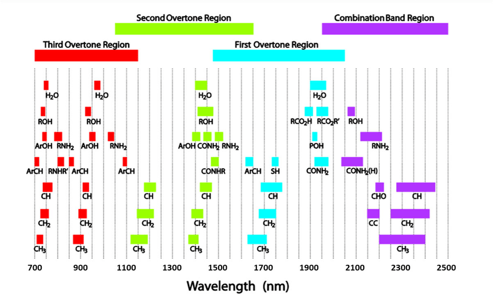
\includegraphics[width=0.75\linewidth]{Images/principle_bands.png}
    \caption{Principal analytical bands and relative peak locations for absorptions in the near-infrared region.\cite{UseInfraredSpectroscopyjohnson2023} Unique absorptions found in the majority of chemical and biological products can be utilized in both qualitative and quantitative examinations.}
    \label{fig:principle_bands}
\end{figure}

Ethanol and water have characteristic NIR spectrum patterns that allow for their identification and quantification as seen in \autoref{fig:anton_paar}. Ethanol has a unique narrow peak at $1200$ nm representing the second overtone of the \ce{C-H} stretching vibration.\cite{InfraredSpectroscopyNIR} Water, on the other hand, shows a flat behaviour at this wavelength due to the lack of \ce{C-H} bonds. 

The intensity of NIR absorption bands is $10-100$ times lower than that of the equivalent basic mid-IR absorption bands.\cite{PracticalGuideInterpretiveworkman2007} This facilitates the direct analysis of strong absorbances and high light-scattering efficiency. Band overlap and penetration depth reduce in the near-infrared (NIR) spectral region, whereas the efficiency of light scattering and absorptivity improves with wavelength. As NIR spectroscopy depends on light absorption, spectral data can be acquired either in transmittance or reflectance mode. Diffuse reflectance $(\log \frac{1}{R} )$ measurements are favored for opaque or light-scattering matrices whereas translucent samples used transmittance $(\log \frac{1}{R})$.

\begin{wrapfigure}{r}{0.5\textwidth}
    \centering
    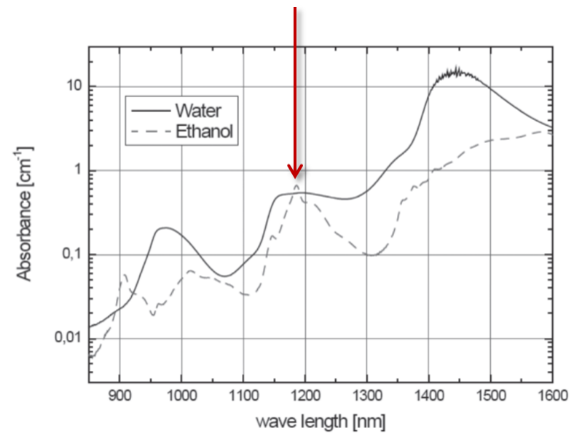
\includegraphics[width=0.48\textwidth]{Images/anton_paar.png}
    \caption{NIR spectrum of ethanol and water \cite{InfraredSpectroscopyNIR}}
    \label{fig:anton_paar}
\end{wrapfigure}

NIR spectroscopy's quickness, adaptability to a variety of materials, and capacity to examine liquid samples make it a promising tool for bio applications.\cite{NearInfraredSpectroscopyBioApplicationsbec2020} Recent advancements are making NIR spectroscopy more accessible with portable handheld instruments that allow for real-time, on-site examination. 
Cell culture media (CCM) plays a vital role, directly impacting process yield and product quality.\cite{CellCultureMediaryder2018} CCM's primary objective is to create and sustain an optimal physiological environment for large-scale cell culturing, ensuring cell health and expression of desired Critical Quality Attributes (CQAs). However, it's crucial to recognize that the chemical and physical properties of CCM are sensitive to microbial growth, chemical reactions, and environmental factors like temperature and light. Without sterilization, CCM can rapidly change due to microbial contamination, leading to increased turbidity and light scatter, consequently elevating baselines and noise in spectra, potentially compromising measurements. While chemometrics can mitigate some measurement errors, identifying errors induced by samples and measurements in CCM analysis can be challenging.

NIR spectra are known to be high-dimensional data due to the baseline drift and other noise signals present. This results in the need for preprocessing techniques for noise filtering and dimensionality reduction before analyzing the true compound signals.\cite{1DConvolutionalNeuralkrohling2023} Hence,  NIR spectra usually involve the use of chemometric algorithms like partial least squares regression (PLSR) and support vector regression (SVR) to clean the data from baseline drift as well as to understand the chemical changes in the samples.\cite{NIRSpectroscopyCombinedshang2023,LinearSupportVectornaguib2014} These algorithms require trained individuals to obtain the necessary parameters used to analyze the spectra.\cite{QuantitativeAnalysisYeastwang2017} Similarly, chemometric models are often limited by their inability to generalize for variance in spectra from different instruments, or changing storage and growing conditions. Deep Learning\cite{ReviewEvolutionChemometricswalsh2023} Machine Learning (ML) can be used to automate extracting the main compound features from high-dimensional spectral data and eliminate the need for feature-selection techniques. 
While different classes of ML algorithms have successfully achieved the classification of NIR spectra,\cite{1DConvolutionalNeuralkrohling2023} traditional ML methods such as partial least squares (PLS), K-nearest neighbor (KNN), and principal component analysis (PCA) require a higher level of expertise to design suitable features of the models architecture.\cite{zhangReviewMachineLearning2022} Deep learning, on the other hand, does not require a high level of expertise as it utilizes the raw features of data to analyze and classify it as needed. This is achieved through multiple hidden layers that are trained end to end. Some of these layers can be specialized convolution layers that allow for the learning and identification of local feature patterns. This aspect enables deep learning architectures to employ less preprocessing for high-dimensional data.\cite{FastDeepLearningyue2021} 

Convolutional neural networks (CNNs) are a class of deep neural networks commonly used for data analysis due to their successful results in image processing and classification,\cite{AnalysisConvolutionalNeuralsharma2018} speech recognition,\cite{SpeechRecognitionUsingalsobhani2021} and other computer vision tasks. CNNs are a feed-forward multi-layer architecture in which a kernel or filter takes specific features from local regions from the upper layer. This architecture allows for an autonomous extraction of important features from complex data for analysis and learning.\cite{NIRSpectroscopyCombinedshang2023} A common drawback of the use of CNNs for spectral analysis is the requirement of large data sets during the training process of the model.\cite{zhangNearInfraredSpectralCharacteristic2022} To avoid overfitting due to a limited number of data samples, one-dimensional CNN (1D-CNN) can be used. These models are similar to traditional CNNs except for the data size required and low computational requirements. 1D-CNNs have proven to have good information extraction and high classification accuracy with simple preprocessing techniques. It has been applied by Shang et al.\cite{NIRSpectroscopyCombinedshang2023} for the analysis and classification of NIR spectra from breast cancer tissue to aid in cancer diagnosis, demonstrating a $94.67\%$ classification accuracy. Chai et al.\cite{Improved1DConvolutionalchai2021} also developed an improved 1D-CNN structure to discriminate Anoectochilus roxburghii from its counterfeits using NIR spectra.

Previous studies performed on 1D-CNN for the analysis of NIR spectral data demonstrate the viability of its application for the online analysis of culture media. The present study aims to develop a method based on NIR spectra acquired on a portable device, as a non-destructive, online method to assess quality attributes of culture media. Due to the expected nature of the data collection, it was necessary to employ a time series analysis when designing the CNN structure. Within this experiment \emph{S. cerevisiae} was used as the model, testing it under two conditions, normal and contaminated with Lactic Acid Bacteria. \emph{Lactobacillus rhamnosus} was used as the contaminant of choice due to its improved growth in the presence of \emph{S. cerevisiae}. Also, using this species ensures the proper growth of \emph{S. cerevisiae} as it remains unaffected in its presence.\cite{YeastHumanCoevolutionnenciarini2024} The NIR spectra of ethanol were analyzed in each case and passed to the deep learning model which classified the “normal” baseline against a “non-normal” sample. 

\section{Methodology}
\subsection{NIR Housing Design}

Due to the design of the DLP NIRscan Nano (Texas Instruments) and the location of the sensor window on the unit, it required a housing to be designed. This housing was designed to both hold the NIR as well as the sample to ensure consistent scan conditions. The housing was created using a 3D printer (P1S, Bambu Labs) using Matte PLA filament (Bambu Labs) for the test models, and was reprinted in ABS filament (Bambu Labs) for the final housing.

The housing underwent multiple iterations with all design and modeling performed within AutoDesk Fusion360 parametric CAD software.\cite{Fusion360} The final iteration of the housing used can be seen below in \autoref{fig:nir_housing}. All of the components slide along a single dovetail mount along the bottom plate to allow for quick assembly while keeping all components secure. Due to slight problems with temperature regulation, a NF-A4x10 5V PWM fan from Noctua was added in addition to a fan speed controller (NA-FC1), to prevent the NIR from overheating during scans. A cuvette holder was also designed to allow for the quick change of samples, while also ensuring that the cuvette remained fixed in place for scans.

\begin{figure}[!h]
    \centering
    \begin{subfigure}[b]{0.4355\textwidth}
        \centering
        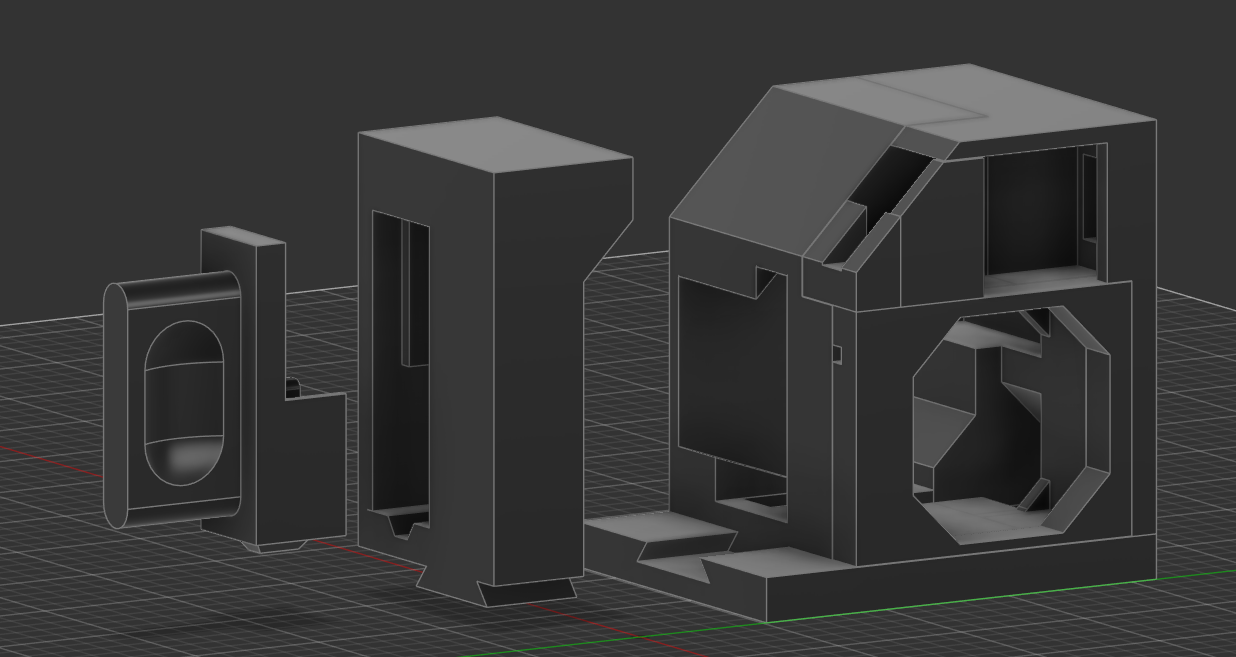
\includegraphics[width=\textwidth]{Images/nir_housing.png}  % Replace with your image file
        \caption{NIR Housing}
        \label{fig:nir_subfig1}
    \end{subfigure}
    \hfill
    \begin{subfigure}[b]{0.551\textwidth}
        \centering
        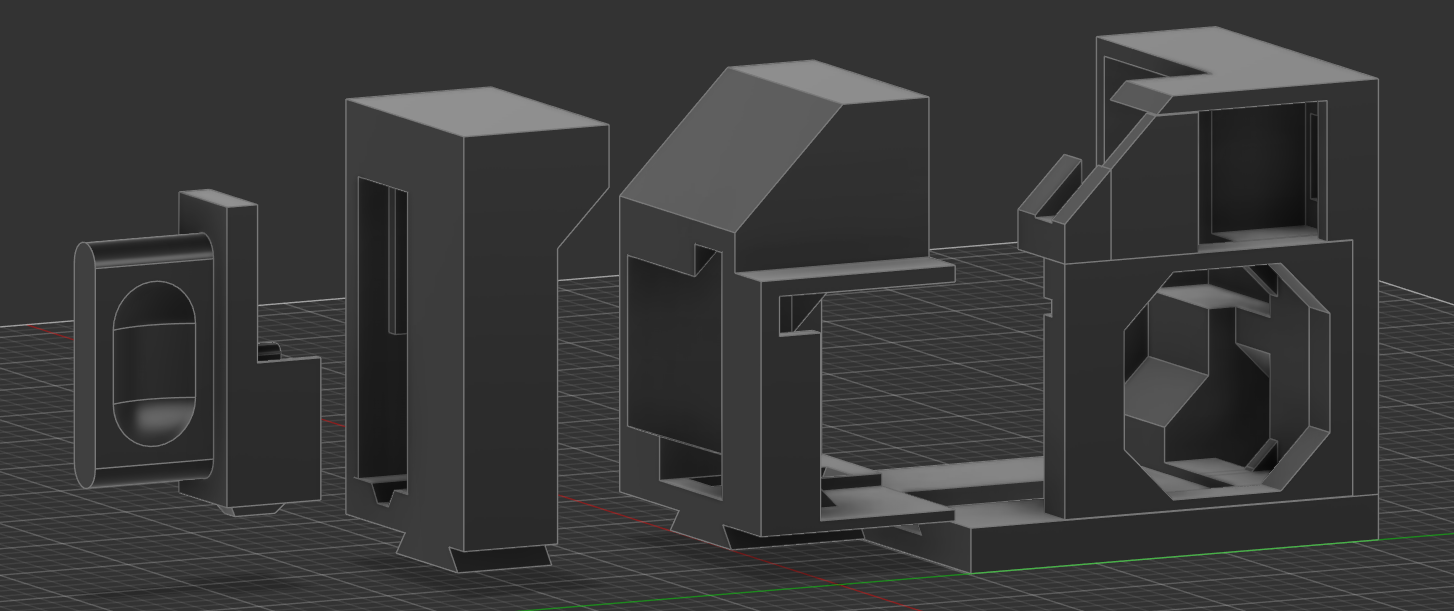
\includegraphics[width=\textwidth]{Images/nir_exploded.png}  % Replace with your image file
        \caption{NIR Housing Exploded}
        \label{fig:nir_subfig2}
    \end{subfigure}
    \caption{NIR Housing Design}
    \label{fig:nir_housing}
\end{figure}

The white PLA background was not as reflective as originally theorized, so the use of Teflon (PTFE) was considered. A high-reflectance PTFE sheet with 3M Adhesive backing was purchased from ThorLabs. This sheet has a reflectance $(> 90\%)$ in the UV spectrum,\cite{HighReflectancePTFESheetsthorlabs} and is one factor attributed to improving the signal-noise-ratio (SNR) within the scans.

\subsection{Ethanol Standard Curves}

To confirm the proof of concept of the project, ethanol standard curves were created and detected using the NIR to determine the differences in signals between different concentrations of ethanol. $6$ solutions of varying ethanol concentrations were tested in two stages, at higher concentrations and low concentrations. For the first standard curve, $300\text{mL}$ of distilled water was retained in a large beaker. Five, $100\text{mL}$ beakers were set up and labelled according to the scheme in \autoref{table:app_ethanol_water_high}. These volumes were added to each beaker and 3mL were subsequently taken out and placed into a plastic cuvette. The cuvette was cleaned with a kimwipe and then placed in the NIR to take a reading. The process was repeated for all beakers 3 times to generate 3 replicates for each sample. The concentrations used were far enough so it would make it easier to tell a difference between the absorbance readings taken from the NIR.

\begin{comment}
\begin{table}[!h]
    \centering
    \begin{tabular}{c c c}
    \toprule
    Sample & Ethanol Volume (mL) & Distilled Water Volume (mL) \\
    \midrule
    1 & 0   & 100 \\
    2 & 25  & 75  \\
    3 & 50  & 50  \\
    4 & 75  & 25  \\
    5 & 100 & 0   \\
    \bottomrule
    \end{tabular}
    \caption{Ethanol and Distilled Water Volumes for Initial Standards}
    \label{table:ethanol_water_high}
    \end{table}
\end{comment}

For the second curve, smaller concentrations of ethanol were used to see if the NIR was able to detect small differences in concentrations of ethanol. The process was similar to the first standard curve. In this case, $600\text{mL}$ of distilled water was retrieved in a beaker and six, 100mL beakers were set up and labelled according to the scheme in \autoref{table:ethanol_water_low}. The remainder of the process was the same as before with the labelled volumes being added to each beaker and $3\text{mL}$ extracted to be placed in a plastic cuvette. The NIR spectra was taken and the process was repeated 3 times to generate 3 replicates. 

\begin{table}[!h]
    \centering
    \begin{tabular}{c c c}
    \toprule
    Sample & Ethanol Volume (mL) & Distilled Water Volume (mL) \\
    \midrule
    1 & 0   & 100 \\
    2 & 1  & 99  \\
    3 & 2  & 98  \\
    4 & 3  & 97  \\
    5 & 4 & 96   \\
    6 & 5 & 95   \\
    \bottomrule
    \end{tabular}
    \caption{Ethanol and Distilled Water Volumes for Low Concentration Standards}
    \label{table:ethanol_water_low}
    \end{table}

\subsection{Yeast Culture}

\subsection{\emph{Lactobacillus} Viability Test}

The Lactobacillus Rhamnosus viability test was conducted at the beginning of the term before running the experiments to ensure that the bacteria were alive when it came time to test the contaminated samples. This was performed by initially sterilizing the environment by lighting a Bunsen burner on an absorption mat. Then four MRS agar plates were inoculated with bacteria from the frozen samples from the previous term using an inoculating loop. Two samples each were taken from the hyperconcentrated and normal concentration samples, and one MRS plate was left untouched to serve as the control. The cells were evenly spread throughout the plate using a cell spreader to ensure even growth and the plates were then closed and wrapped with parafilm. They were then incubated at 37°C for 24 hours to allow for the bacteria to grow. 

\subsubsection{Lactobacillus Plating}

To prepare the contaminated cultures, a sterile environment was created by lighting a bunsen burner on an absorption mat, after which a hyperconcentrated sample of lactobacillus was retrieved from the freezer. An inoculating loop was used to pick up bacteria from the sample and placed on an agar plate, after which a cell spreader was used to spread the bacteria evenly across the plate. A second agar plate was also retrieved to serve as a control. Once the colonies were evenly spread the plate was closed, wrapped with parafilm and placed in an incubator for 24 hours at $37^{\circ}C$. After the incubation, the plate with lactobacillus was retrieved, and an inoculating loop was used to pick up colonies and place them in 20mL of YPD in an erlenmeyer flask. Afterwards, the flask was placed in a shaking incubator for 48 hours at $37^{\circ}C$. After 2 days the sample had reached confluency and 500uL were placed in test tubes after which the remaining was filled with YPD to reach a final volume of 3mL. The samples were then labeled and placed in the freezer at $-20^{\circ}C$ until they were needed for contaminated runs,   

\subsection{Spectral Measurement}

\begin{table}
    \centering
        \begin{tabular}{l c}
        \toprule
        Variable & Setpoint\\
        \midrule
        Start wavelength (nm): & $900$ \\
        End wavelength (nm): & $4.68$ \\
        Pattern Pixel Width (nm): & $1500$ \\
        Exposure (ms): & $1.27$ \\
        Digital Resolution: & $264$ \\
        Scan Repeats: & $9$ \\
        PGA Gain: & $64$ \\
        \bottomrule
        \end{tabular}
        \caption{Scan Setting for DLP NIRScan Nano}
        \label{tab:scaninfo}
\end{table}

\subsubsection{Spectral Processing}

Hadamard Transform is one of the available protocols built into the DLP NIRscan Nano. Unlike the column protocol which only reads one wavelength at a time, the Hadamard protocol takes a multiplex scan of multiple wavelengths simultaneously. An algorithm is then used to decode the individual wavelengths from the multiplex scan. The benefit of using Hadamard over Column is that Hadamard has a much better signal-noise ratio which will minimize the required preprocessing later.

\subsection{Data Pipeline}

Due to the limited number of samples that were able to be collected, the data was augmented for the sake of training. Different data augmentation methods were explored to best fit our use case. Factors such as simplicity, and reducing the risks of overfitting were considered. The use of subsampling was determined to be the optimal method and was applied to future data collection.

\subsection{Subsampling}
The data augmentation pipeline that was created is based on a type of subsampling called cyclic subsampling. Cyclic subsampling divides the dataset into non-overlapping subsets using an offset starting index and a set interval. This method has a few key features that make it optimal for this dataset when compared to other methods like temporal subsampling with sliding windows or random sampling. Since the interval remains the same across all subsamples, the temporal order of the dataset can be maintained when training a neural network. The non-overlapping sub-samples have a lower redundancy within the datasets compared to other methods, which will help prevent overfitting. The improved diversity would also allow the model to account for variations in starting time or time accumulation from scan duration.

Using cyclic subsampling had some major considerations that changed future data collection. The subsample interval would have to be large enough to prevent redundancy, while also remaining small enough to not create a large margin of error within the model. The frequency of scans would also have to be high enough to prevent the offset time points from approaching the cycle interval. Due to these considerations, our scanning frequency was changed to 60 second intervals. Our default augmentation parameters were set at a 60 second offset with a 15 minute (900 second) cycle interval with 3 subsamples per dataset. The model was tested using the default parameters as well as increasing the number of subsamples to 5, 6, and 7.

\subsection{Normalization and Scaling}
In addition to subsampling the data, the samples underwent additional processing. The only processing step originally implemented was scaling/normalization. There were multiple normalization methods integrated into the pipeline with global max/min normalization and Scikit Learn MinMaxScalar. The purpose of this processing step is to scale all of the data between 0 and 1 in order to better observe the key features within the same range. MinMaxScalar uses the formula found in \autoref{eq:minmax}, which scales the data after the data is normalized using the global max/min method. 

\begin{equation}
    X_{\text{scaled}} = \frac{X - X_{\text{min}}}{X_{\text{max}} - X_{\text{min}}} \times (f_{\text{max}} - f_{\text{min}}) + f_{\text{min}}
    \label{eq:minmax}
\end{equation}

\subsection{Gaussian Noise}
To prevent the model from overfitting, Gaussian noise was added into the datasets. This was done using Numpy’s random.normal function which takes a mean, a standard deviation, and data size as arguments (Numpy.Random.Normal — NumPy v2.0 Manual, n.d.). The function then draws values based on Gaussian distribution. The output array of the normal values is then added to the current dataset. The pipeline was set to utilize a mean of 0, with a standard deviation of 0.005

\subsection{Convolutional Neural Network}

The classification of near-infrared (NIR) spectra to determine the contamination state of liquid media was performed with a one-dimensional convolutional neural network (1D-CNN). This neural network model uses the Keras library with Tensorflow as the backend. The use of Keras facilitates the modelling of the CNN due to its intuitive and user-friendly interface.\cite{kerasteam_keras} The Tensorflow backend allows for accelerated training when used with GPU.\cite{acecloudteam_2024_tensorflow} It also enables a detailed visualization through Tensorboard. Their combination results in a flexible model with easily customizable variables, like the layers and optimizers, along with shorter training times	

\subsection{Model Architecture}

The architecture of the model employs five different layers repeated at different points, as shown in \autoref{fig:cnn_arch}. The model consists of two Conv1D layers, with 64 and 32 filters respectively. These filters allow for the extraction of significant features in the input data.\cite{nisha_2020_applications} These features set the parameters that will be learned throughout training. To avoid overfitting and reduce the dimensionality of these parameters, MaxPooling1D layers and Dropout layers are implemented after the Conv1D layers. The Dropout layer was set to a 0.5 rate, meaning that for each iteration, $50\%$ of the nodes or neurons were ignored to ensure that learning mistakes from other nodes were not fixed by the whole network.\cite{DropoutNeuralNetworksyadav2023} This in turn reduces overfitting and improves the generalization of the model.

The activation function, or function that transforms the input of a node into an output of that node, is a key component of a neural network. The model uses the Rectified Linear Unit (ReLU) function as the activation function, which only outputs non-negative outputs or zeros.\cite{brownlee_2019_a} This is commonly used in CNNs due to its ease of training and superior performance. A final dense layer is implemented with a sigmoidal activation function. This function outputs a probability score between 0 and 1 to determine the contamination state of the sample: 0 for non-contaminated and 1 for contaminated.\cite{saeed_2021_a} 

\begin{figure}[!h]
    \centering
    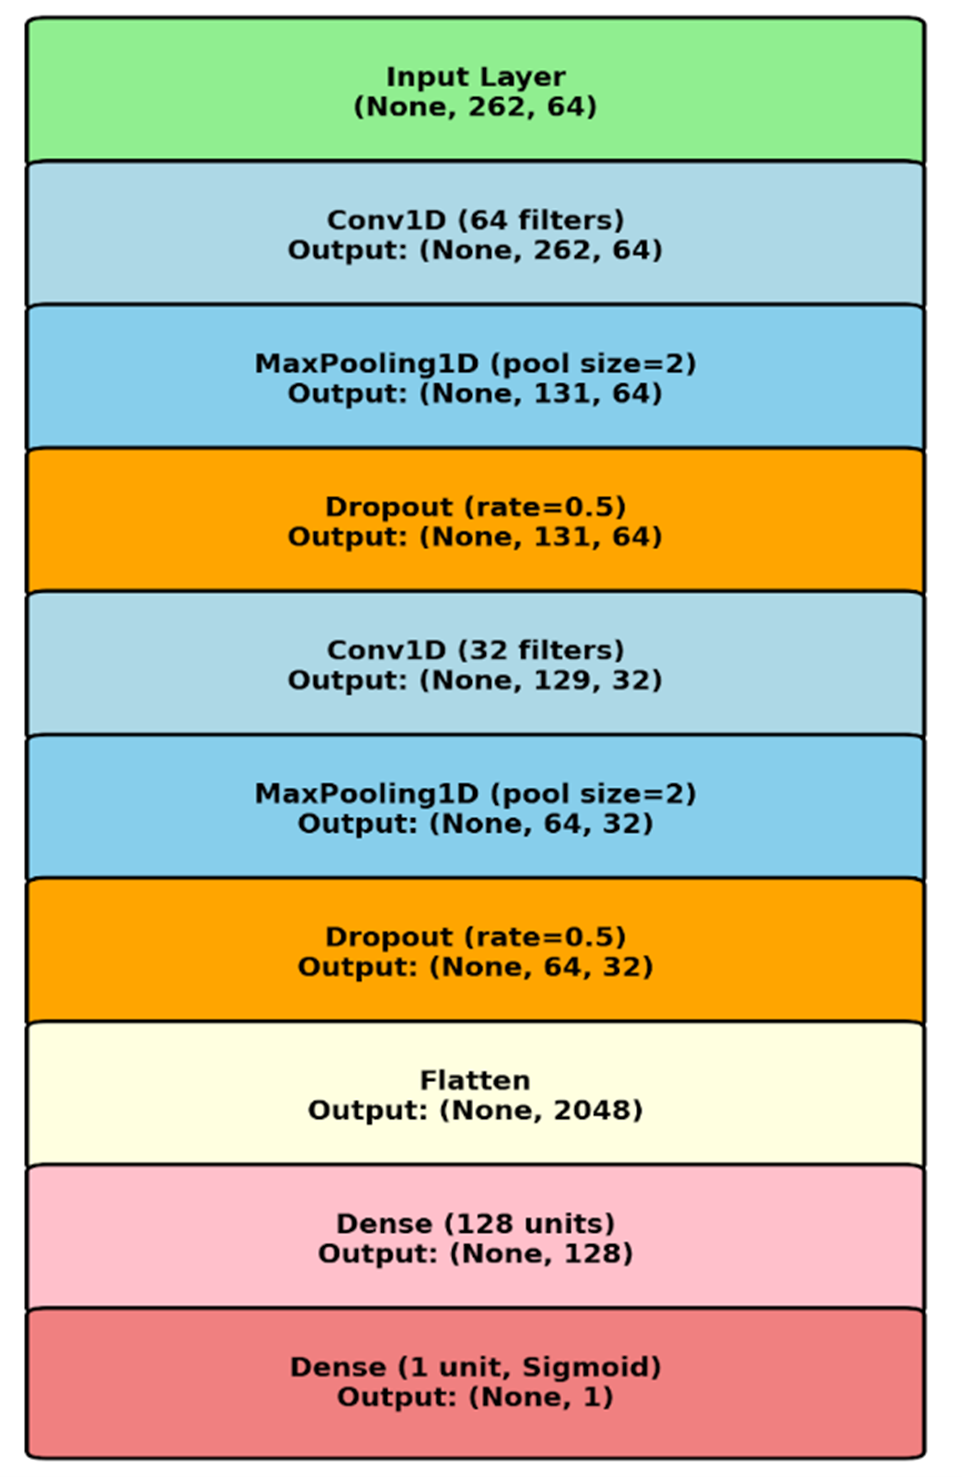
\includegraphics[width=0.4\linewidth]{Images/cnn_arch.png}
    \caption{1D-CNN architecture diagram}
    \label{fig:cnn_arch}
\end{figure}

\subsubsection{Optimizer and Loss Function}
Optimizers are functions responsible for adjusting the parameters as training progresses.\cite{eitcaacademy_2023_what} This is done to reduce the loss function, a mathematical quantification of the error margin between the prediction and the ground truth. The Adam algorithm was chosen as the optimizer. This follows a stochastic gradient descent based on adaptive estimation and regulated by the learning rate.\cite{kerasteam_keras} It allows for the model to reach an optimal point faster without taking large learning steps that could lead to skipping key information during training. The learning rate was set to 0.0005 to avoid reaching a convergence between the ground truth and prediction too early during training.

\begin{equation}
    L = -\frac{1}{N} \sum_{i=1}^{N} \left[ y_i \cdot \log(p(y_i)) + (1 - y_i) \cdot \log(1 - p(y_i)) \right]
    \label{eq:loss_function}
\end{equation}

The binary cross-entropy loss function was used in the model due to the binary classification nature of the project. The loss function is defined in \autoref{eq:loss_function}, where $y$ is the label $(1$ for contaminated and $0$ for non-contaminated$)$ and $p(y)$ is the predicted probability of the point being contaminated for all $N$ points. Binary cross-entropy quantifies the differences between the logarithmic probability distributions and penalizes inaccurate predictions which helps assess the model’s prediction confidence.

\subsection{Training Parameters}
To train the model, a dataset for each class was utilized. The non-contaminated dataset contained a total of 75 samples while the contaminated dataset had 54 samples post-augmentation. The model was trained through a mini-batch gradient descent, which consists of training the model on small random subsets of the training data at each iteration.\cite{MiniBatchGradientajaymehta2023} In this case, the batch size or training subset was set to 16, meaning that for every 16 samples, the model weighted the results for learning.  This allows for a reduction in the computational cost of the model and a faster convergence of the algorithm. Each dataset was split to use $20\%$ of the samples for validation. The splitting was performed by stratified sampling to ensure the training and validation sets had a balanced representation of both classes.

\subsection{Visualization of Metrics}
To permit an easy understanding of the model’s performance, the primary training metrics were visualized using TensorBoard. The loss, accuracy, and learning rate changes were tracked in real time during the training phase. These metrics were used to produce four plots: (1) combined validation loss and accuracy over epochs, (2) confusion matrix, and (3) receiver operating characteristic (ROC) curve. The validation loss and accuracy over the epochs plot show the progression of the training as the number of epochs increases. The validation loss indicates how effectively the model is learning and allows to observe if overfitting or underfitting of the model is occurring. The validation accuracy indicates how well is the model improving its prediction accuracy during the training phase. Including these two metrics for the different folds in the same plot allows for a clear comparison of the improvement of the model as the training iterations increase. The confusion matrix provides a detailed and intuitive visualization of the model’s prediction performance.\cite{AsynchronousEEGbasedBCIhernandez-del-toro2021} It compares the ground truth labels against the predicted labels of the test data, showing the counts for true positives, true negatives, false positives, and false negatives. The ROC curve shows the classifier performance across different thresholds. It requires calculating the true positive rate and the false positive rate at each threshold to plot these together. The resulting area under the curve represents the probability that the model can properly classify between classes. An area under the curve equal to 1.0 represents a perfect model with low random classification. These plots provide an overview of the model performance and allow for the assessment of the training process to identify potential overfitting.

\section{Results}

\subsection{Standard Curves}

The raw NIR spectra for the standard curves showed a clear difference in the peaks as the concentration of ethanol increased. To analyze the results of the graphs, the second overtone of the \ce{C-H} stretching vibration, just before 1200nm, is considered. This overtone is representative of ethanol as it indicates the pronounced symmetrical vibration of the methyl group.

\begin{figure}[!h]
    \centering
    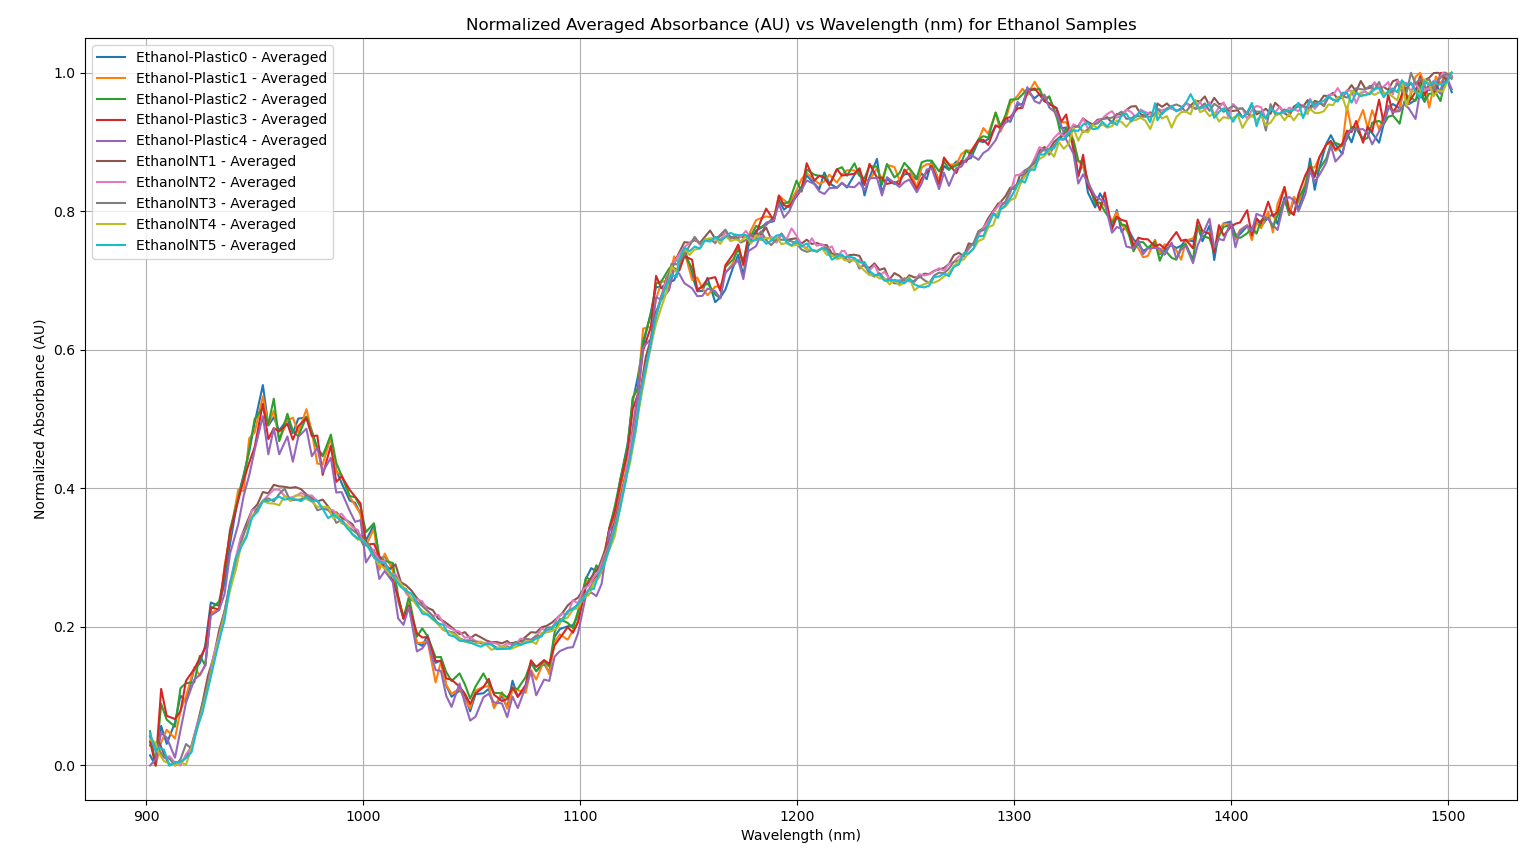
\includegraphics[width=0.75\linewidth]{Images/Ethanol_Standard_PvQ.png}
    \caption{Comparison of ethanol curves (0-5\%) for analysis of cuvette
    material. Curves labelled Ethanol-Plastic(N)-Averaged is Plastic cuvette and
    curves labelled EthanolNT(N)-Averaged is quartz cuvette.}
    \label{fig:eth_pvq}
\end{figure}

\begin{figure}[!h]
    \centering
    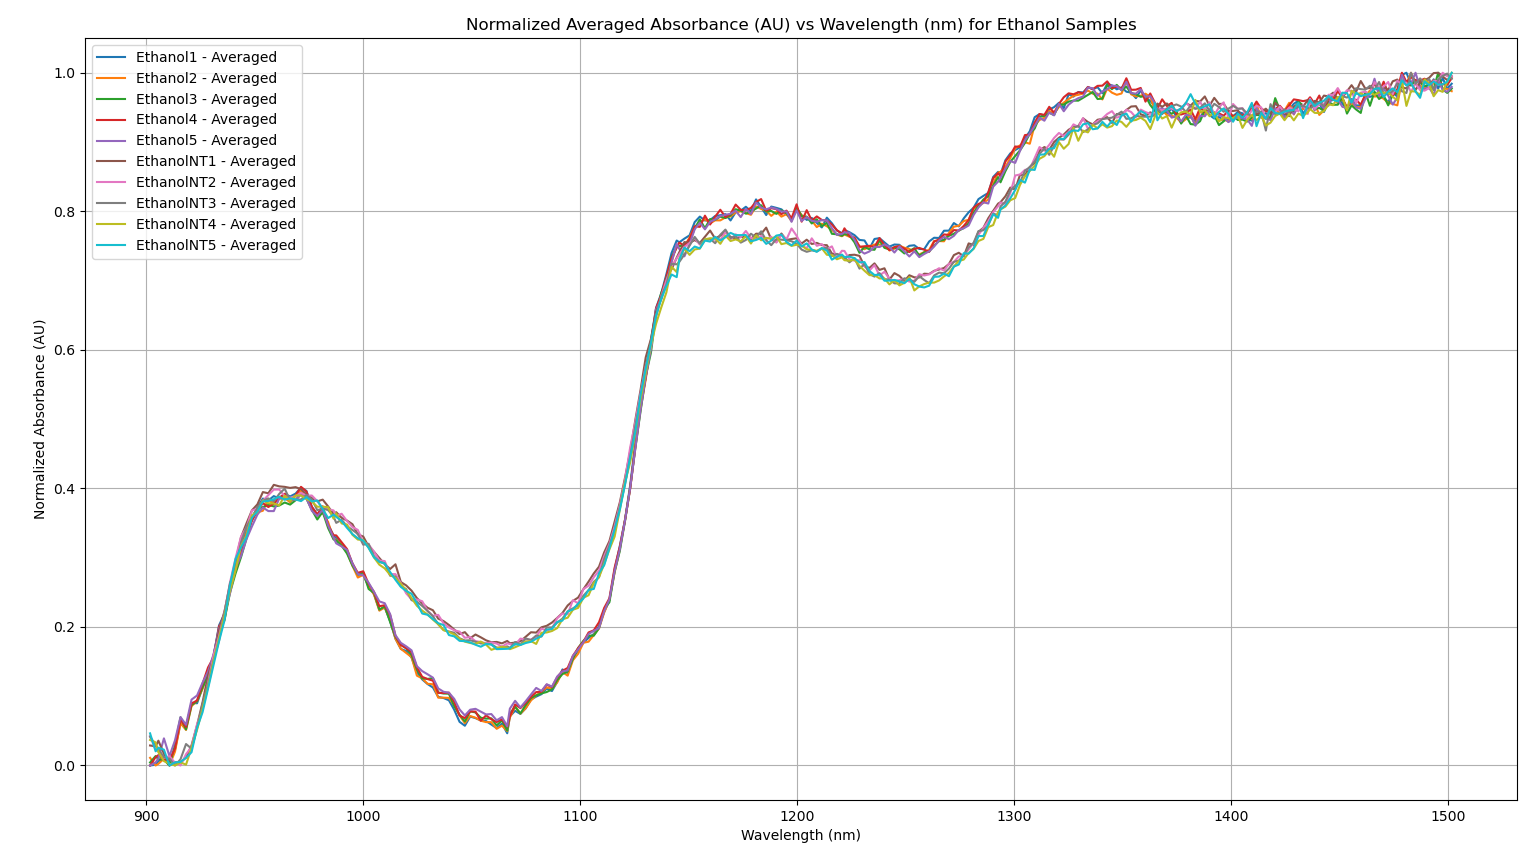
\includegraphics[width=0.75\linewidth]{Images/Ethanol_Standard_Compared.png}
    \caption{Comparison of ethanol curves (0-5\%) for analysis of the
    presence of Teflon.Curves labelled Ethanol(N)-Averaged is with teflon and
    curves labelled EthanolNT(N)-Averaged is without Teflon.}
    \label{fig:eth_comp}
\end{figure}

The use of plastic cuvettes in the initial experiments contributed to suboptimal peak resolution in the NIR spectrometer data. To address this issue, plastic cuvettes were replaced with quartz cuvettes, leading to significant improvements in peak clarity and noise reduction. The results can be seen in \autoref{fig:eth_pvq}, where the smoother curve with less spikes and defined peaks is from utilizing a quartz cuvette. 

The NIR housing is made from Acrylonitrile Butadiene Styrene (ABS), a material chosen for 3D printing due to its ability to withstand the heat generated by the NIR spectrometer. To address light absorption issues and enhance reflectance, Teflon tape was applied to the spectrometer housing to reduce stray light and minimize noise. This modification enhanced the precision of absorbance measurements by reducing light scattering and interference, as seen on \autoref{fig:eth_comp}. As a result, the absorbance curves exhibited smoother transitions and more defined peaks, enabling better visualization and detection of variations in ethanol production during yeast fermentation. These adjustments contributed to the generation of reliable and interpretable data, optimizing the performance of the CNN model.

\subsection{Scans and Processed Samples}

\begin{figure}[!h]
    \centering
    \includegraphics[width=0.75\linewidth]{Images/Sample8_1-n_plot.png}
    \caption{Time-Series plot of Sample 8 after preprocessing}
    \label{fig:non-contaminated-8}
\end{figure}

\begin{figure}[!h]
    \centering
    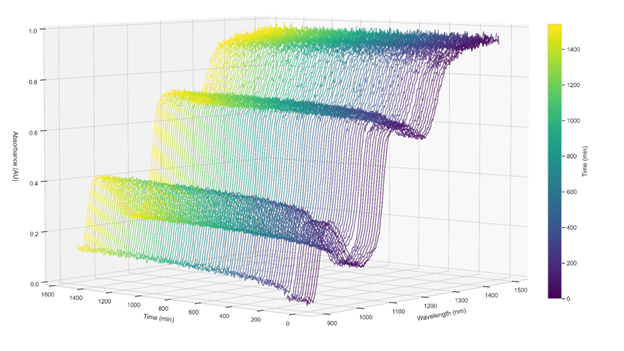
\includegraphics[width=0.75\linewidth]{Images/sample12.png}
    \caption{Time-Series plot of Sample 12 after preprocessing}
    \label{fig:contaminated-12}
\end{figure}

\subsubsection{Spectra Comparison}

\begin{figure}[!h]
    \centering
    \begin{subfigure}[b]{0.49\textwidth}
        \centering
        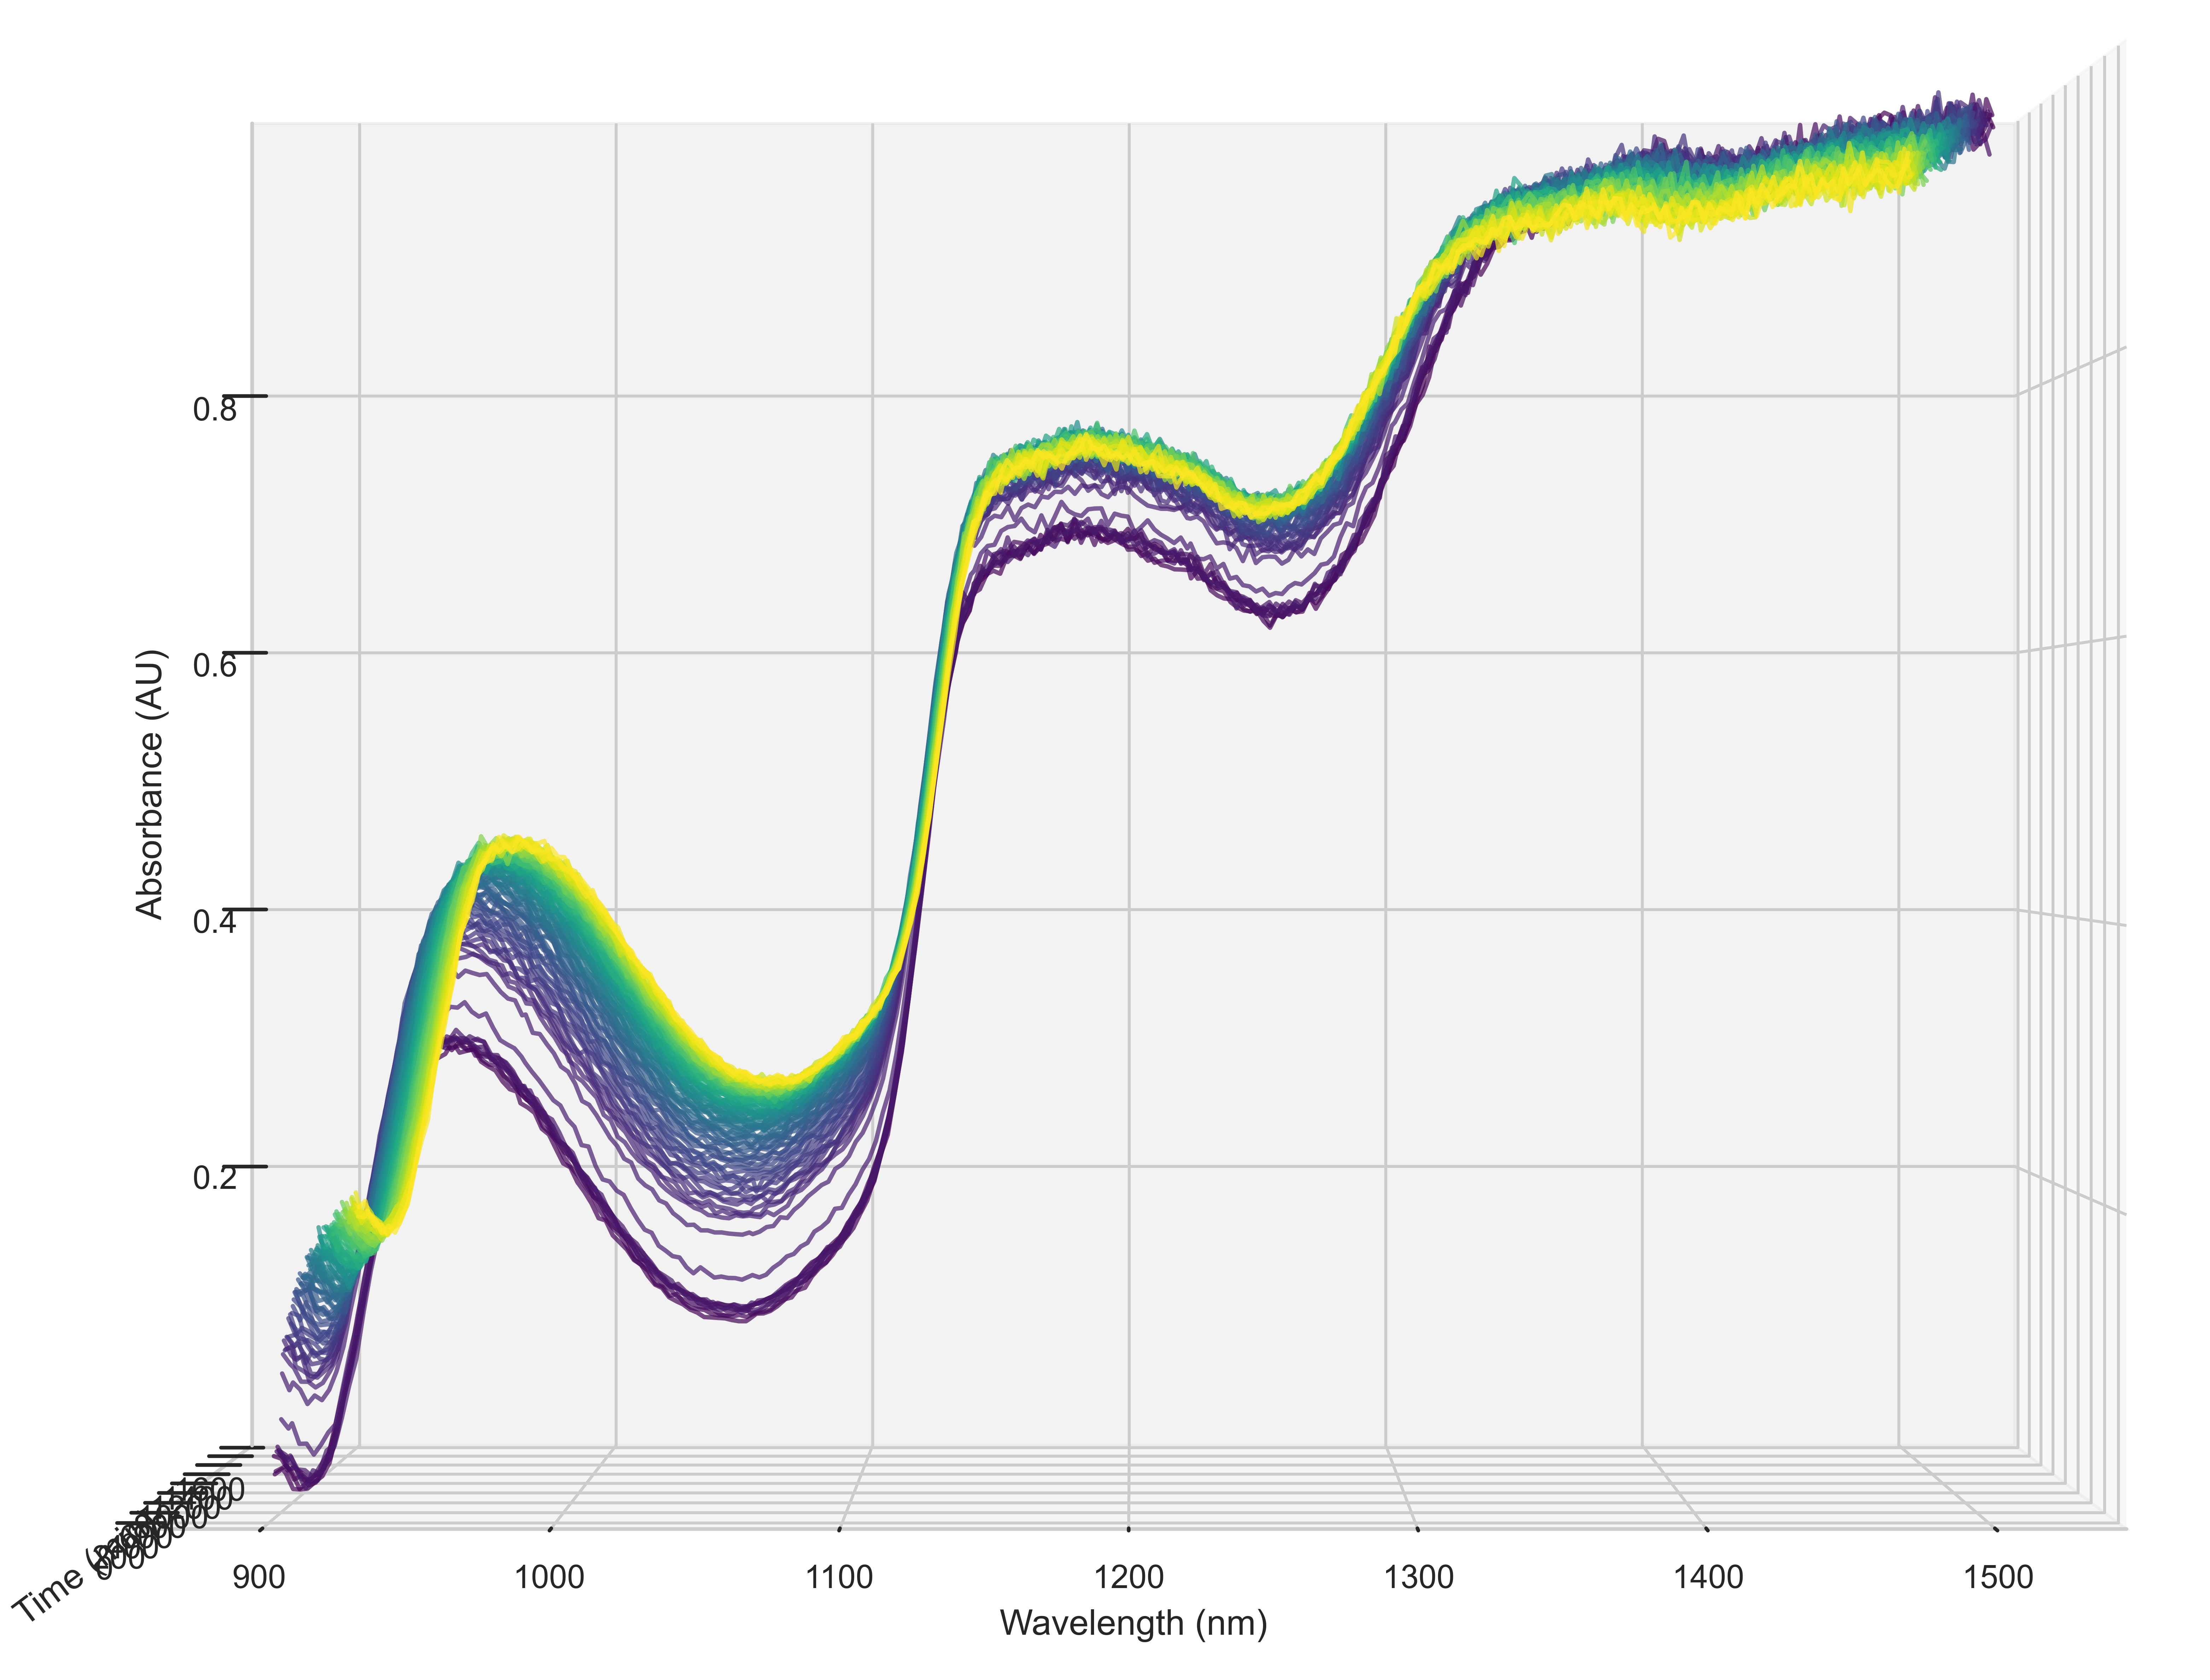
\includegraphics[width=\textwidth]{Images/Sample8_1-n-front.png}  % Replace with your image file
        \caption{Sample 8 (Non-contaminated)}
        \label{fig:sample8-front}
    \end{subfigure}
    \hfill
    \begin{subfigure}[b]{0.49\textwidth}
        \centering
        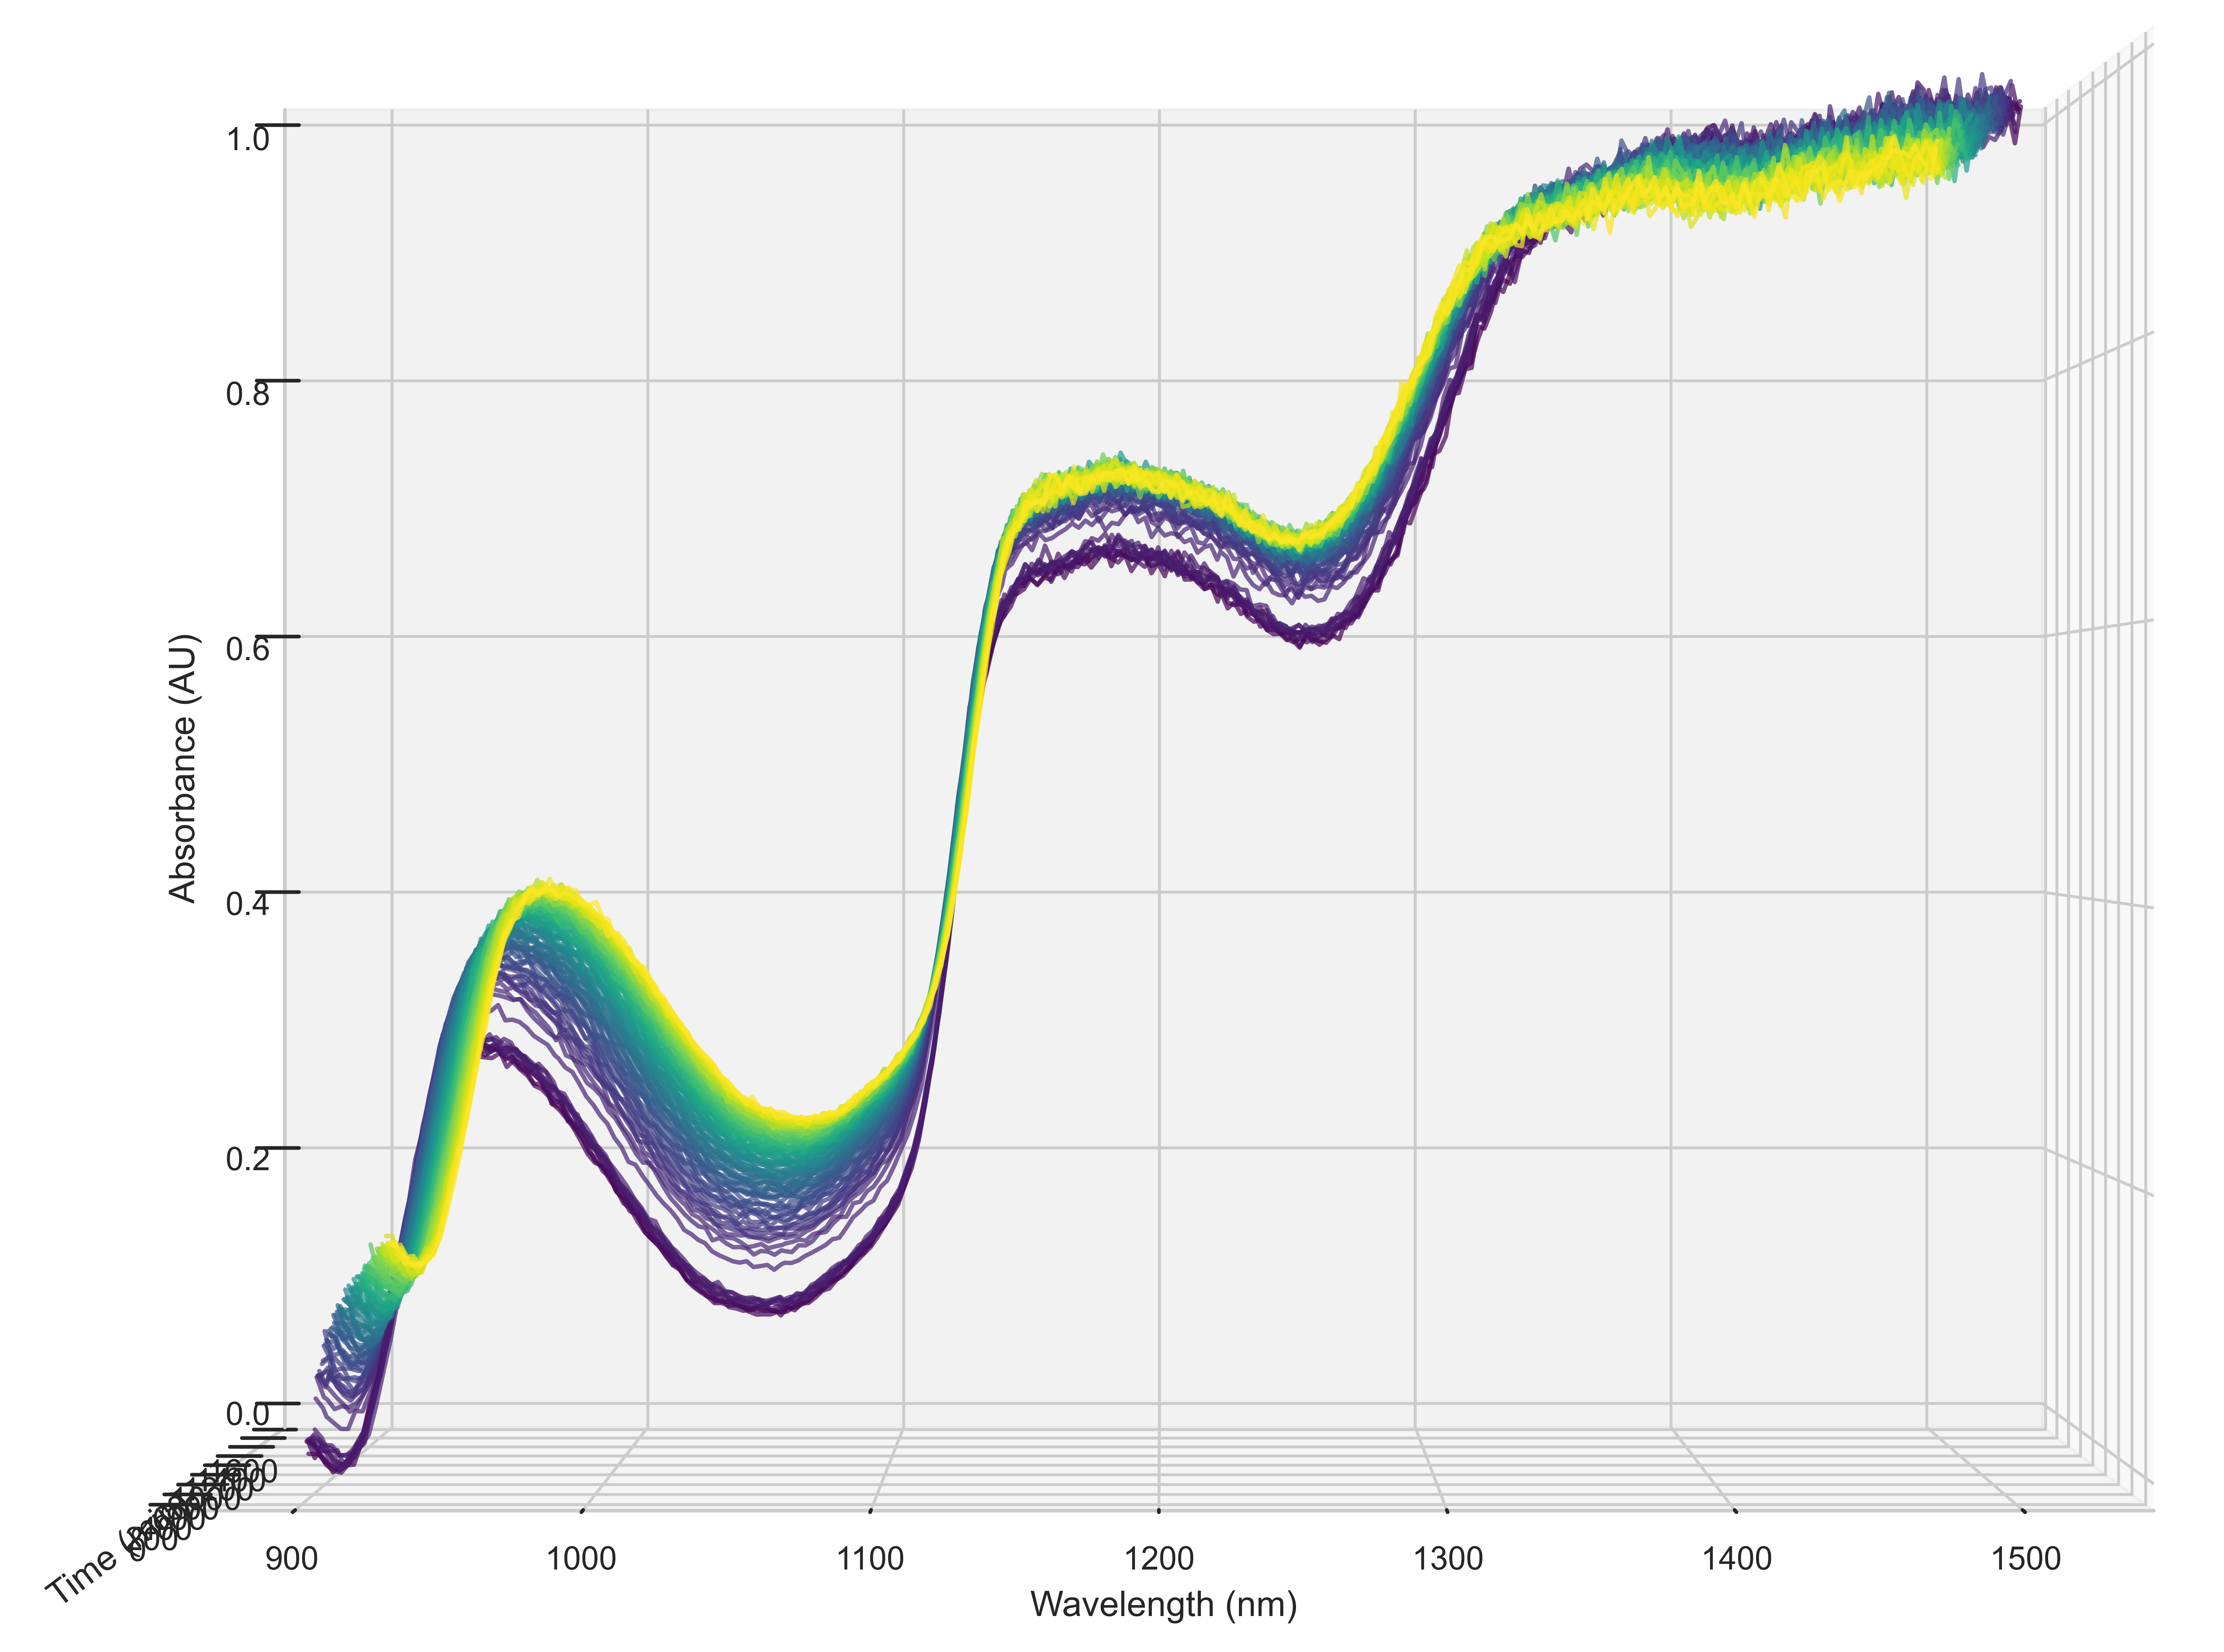
\includegraphics[width=\textwidth]{Images/Sample12_1-n_plot.png}  % Replace with your image file
        \caption{Sample 12 (Non-contaminated)}
        \label{fig:sample12-front}
    \end{subfigure}
    \caption{Comparison of non-contaminated Sample 8 and contaminated Sample 12}
    \label{fig:spectra_comp}
\end{figure}

The non-contaminated and contaminated spectra show noticeable differences between them as seen in Figure x. The contaminated sample shows a lower absorbance in its major peaks between $900-1000$ nm and $1100-1300$ nm. There is also a slight visible right shift of the contaminated spectra compared to the non-contaminated sample. The initial absorbances of the sample were however higher within the contaminated sample. Both samples displayed a subtle drop in absorbance towards the end of the fermentation with the drop being more prominent within the non-contaminated spectra.

\subsection{Model Validation}

The graph in \autoref{fig:val_loss} presents the validation loss and validation accuracy over 50 epochs. The validation accuracy starts at a moderate level and exhibits notable fluctuations during the initial epochs before stabilizing around $90\%$ in the later epochs. The validation loss begins at a relatively high value and steadily decreases throughout the training process, showing a consistent downward trend and reaching a final value of 0.252 by the final epoch. Both metrics display distinct patterns, with accuracy improving and loss decreasing as training progresses, despite the initial fluctuations in accuracy.

\begin{figure}[!h]
    \centering
    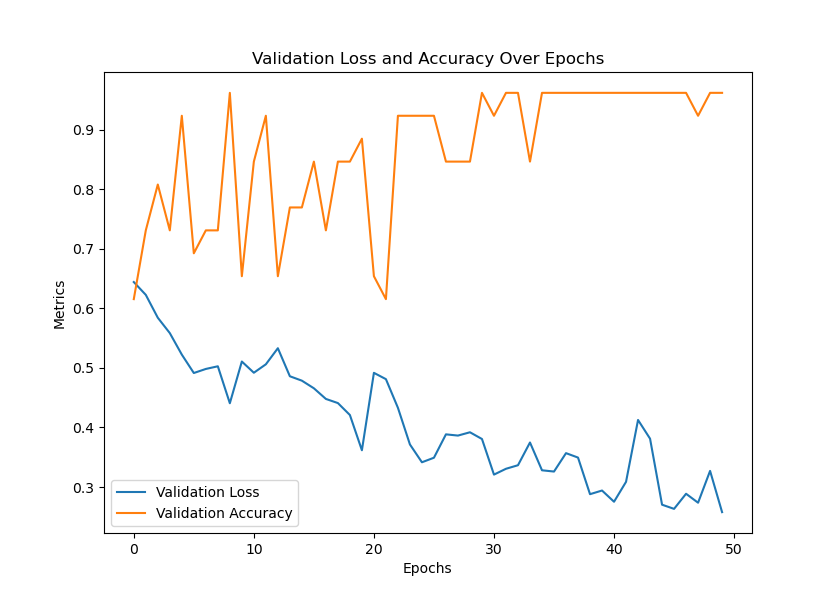
\includegraphics[width=0.75\linewidth]{Images/aa.png}
    \caption{Validation loss and accuracy over epochs}
    \label{fig:val_loss}
\end{figure}

The confusion matrix, shown on \autoref{fig:conf_matrix}, displays the performance of the classification model in differentiating between "Non-Contaminated" and "Contaminated" samples. The matrix shows that the model correctly classified 15 "Non-Contaminated" samples (true negatives) and 10 "Contaminated" samples (true positives). It misclassified one "Contaminated" sample as "Non-Contaminated" (false negative) and made no false positive errors (0 "Non-Contaminated" samples misclassified as "Contaminated"). This highlights a high overall classification accuracy, with the model successfully identifying most of the samples.

\begin{figure}[!h]
    \centering
    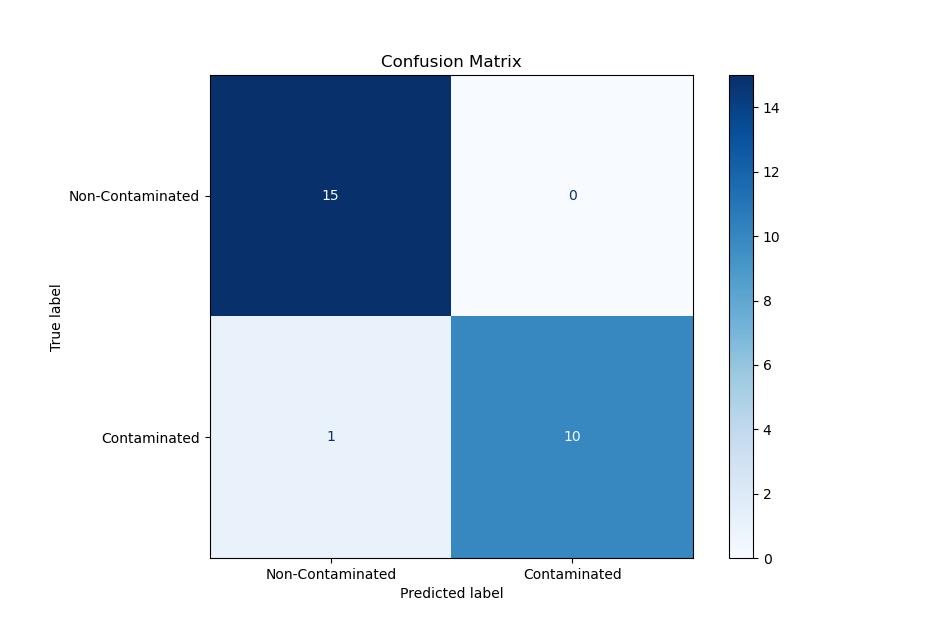
\includegraphics[width=0.75\linewidth]{Images/bb.png}
    \caption{Confusion matrix for validation samples}
    \label{fig:conf_matrix}
\end{figure}

The Receiver Operating Characteristic (ROC) curve in figure 12 demonstrates the performance of the classification model by plotting the True Positive Rate (TPR) against the False Positive Rate (FPR) at various classification thresholds. The ROC curve exhibits a high degree of separation from the diagonal line (random classifier), with an Area Under the Curve (AUC) value of 0.97. This indicates a strong ability of the model to distinguish between the "Contaminated" and "Non-Contaminated" classes.

\begin{figure}[!h]
    \centering
    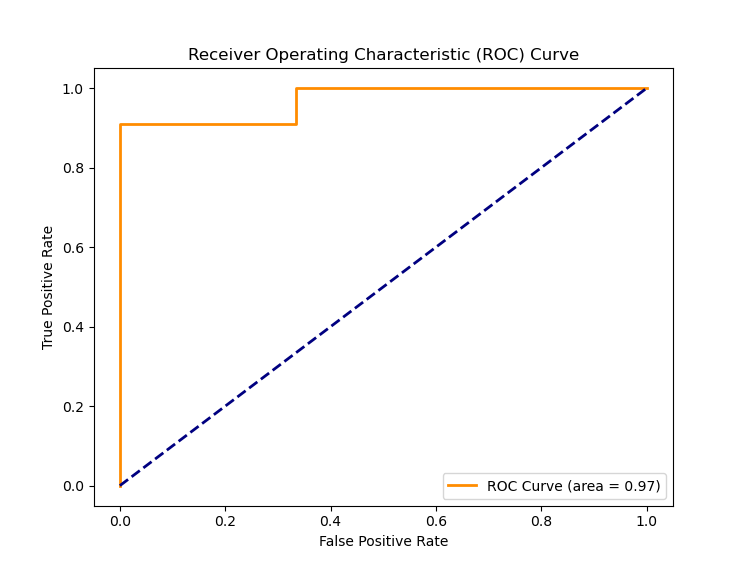
\includegraphics[width=0.75\linewidth]{Images/cc.png}
    \caption{Receiver Operating Characteristic (ROC) curve for the model's validation}
    \label{fig:conf_matrix}
\end{figure}

\subsection{Training Accuracy}

To demonstrate the model’s accuracy during training, the model was trained multiple times with identical conditions except for the validation and training set as established by the random stratified sampling. The different training times demonstrate notable variability across training iterations (Appendix D). Validation loss consistently decreased over epochs in all runs, though both initial and final loss values showed slight differences between iterations. Validation accuracy exhibited fluctuations, with some iterations showing more stable improvements while others experienced greater variability in trajectory and peak values. The confusion matrices reveal variations in classification outcomes across runs, with discrepancies in the number of true positives, true negatives, false positives, and false negatives. Certain runs achieved higher true positive rates and fewer false negatives, while others showed increased misclassifications, particularly in the "Contaminated" class. ROC curves further highlight the variability in classification performance, with AUC values ranging from 0.90 to 0.99. These differences indicate that while the model consistently performs well overall, the extent of its robustness and discrimination ability depends on the specific composition of the validation set resulting from stratified sampling.

\section{Discussion}

\subsection{Ethanol Curves}

A detailed analysis of the results from experiments that were previously carried out revealed that the peaks observed from the NIR spectrometer were not sufficiently distinct to accurately identify the presence of ethanol. To improve the accuracy of the CNN model, and ensure that the data is reliable, the peaks had to be observed with less noise and be clearly distinct. The use of plastic cuvettes was identified as a factor that contributed to the suboptimal peak resolution. This issue was addressed by replacing the plastic cuvette with a quartz cuvette for data collection runs. 

Quartz cuvettes are highly durable and resistant to scratches, thereby being an ideal material to run experiments frequently whereas plastic cuvettes have to be discarded after a single use (Cuvettes for Spectrophotometer, 2023). Moreover, quartz has the least path length variation when compared to alternate materials like glass and plastic, ensuring that the results collected were consistent and reproducible. Another key advantage is quartz’s ability to withstand high temperatures, which is essential for extended NIR spectroscopy experiments. Since scans were taken every minute for 24 to 48 hours, the spectrometer generated significant heat, and quartz cuvettes could endure these conditions without compromising performance.

On the other hand, the quartz cuvette did have a high initial cost. Since the benefits outweigh the drawbacks, the quartz cuvette was our choice of material to replace plastic.

Teflon tape was applied to the housing of the spectrometer to improve the quality of NIR spectroscopy measurements and minimize noise. Placing the tape at the rear of the cuvette absorbed stray light rays that would otherwise cause scattering and distortion, thus improving the precision of the absorbance readings. This adjustment reduces interference and ensures a more stable light pathway, allowing the spectrometer to capture a broader and more consistent range of absorbance values.

The resulting absorbance curves exhibit smoother transitions, with well-defined dips that reflect the dynamics of the yeast fermentation process more clearly, free from erratic fluctuations. The gradual slopes and smooth dips contribute to a more refined and optimal spectral output, enabling subtle variations in ethanol production to be more accurately detected. This improvement in the clarity and aesthetics of the spectral curves enhances both the interpretability and the visual appeal of the scans, ultimately supporting more precise data analysis.

\subsection{Spectra Analysis}

A lot of the final samples gave very promising results based on their graphs. The use of colour gradients on the graphs allows the observation of the time-series dimension within the results. Figure x and Figure x are the spectra graphs of Normal and Contaminated Sample 8 and 12 respectively. Both show an average growth of the entire spectra over the course of a large portion of the data collection period. Both the contaminated sample and normal show a growth in the expected second overtone \ce{C-H} stretch between $1150-1200$ nm which can be attributed to an increase in ethanol concentration. \autoref{fig:spectra_comp} shows \autoref{fig:contaminated-12} and \autoref{fig:non-contaminated-8} compared in order to get a better representation of the scale between the two sets of spectra. This graph shows that the Contaminated sample had larger increases in its absorbance between $950-1100$ nm while the Normal sample had larger increases between $1150-1500$ nm. 

All of the observed non-contaminated samples have a slight inconsistency in the collected data. After a certain period of time the overall absorbance began to decrease towards the original absorbance at time 0. Some wavelengths continued to even drop below the original absorbance. This can be especially seen in \autoref{fig:spectra_comp} above 1350 nm. These inconsistencies will continue to be explored in future, however there currently is not enough data to determine the exact cause of this.

\subsection{Model Results}

The results from the validation metrics, confusion matrices, and ROC curves demonstrate the model's strong performance in distinguishing between "Contaminated" and "Non-Contaminated" samples, with validation loss reaching as low as 0.252 and accuracy stabilizing above 0.9. Despite initial fluctuations in accuracy, the model generalizes well on the validation data, achieving consistently high AUC values and minimal misclassifications. These findings highlight the model’s robustness and effectiveness even when trained on a limited dataset, comprising 75 "Non-Contaminated" and 54 "Contaminated" samples post-augmentation.

The variability observed across training runs, despite identical model configurations, highlights the impact of stratified sampling on model performance. Differences in the distribution of validation samples resulted in slight variations in confusion matrices and ROC curves. While most runs maintained high true positive rates and low false positive rates, discrepancies in false negatives highlight potential areas for improvement, particularly for applications requiring high sensitivity.

Overall, these results validate the model's robustness and effectiveness for the classification task. However, given the limited dataset size, future efforts should focus on augmenting the dataset with additional samples to improve generalizability and reduce sensitivity to validation set composition. Other techniques such as k-fold cross-validation should be evaluated and tuned to further ensure consistent and reliable performance of the model. These findings emphasize the importance of expanding the dataset and implementing comprehensive validation strategies to enhance the model's stability and reliability in practical applications.

\subsection{Future Steps}

For the continuation of the project, two main activities are proposed to improve the model’s performance: further non-contaminated and contaminated data collection, and working on the data pipeline. 

The use of strategies such as single-class training and K-Fold cross-validation was based on the need to use the limited data set as efficiently as possible for both training and validation of the model. While the augmentation of the data was beneficial in increasing the dataset from the original data collected, the model’s performance results could be improved by increasing the number of contaminated and non-contaminated datasets. This will allow for a comprehensive multi-class training model that is capable of a more accurate classification. Regularization methods could also be considered to reduce the overfitting of the model. 

In addition, the deep learning model can be exported and integrated with a real time pipeline on the same computer as the NIR to allow the model to run in real time. The model could be adjusted so that it would be based on time point instead of the total sample and this would allow it to be used while a sample is running. This would allow for the user to detect real-time contamination and determine if a run can be stopped prematurely so as to save time and resources. 

\section{Conclusion}

NIR spectroscopy was optimized to monitor ethanol production in yeast fermentation by addressing initial challenges with sharpness and noise in the absorbance curves. Quartz cuvettes replaced plastic ones to enhance light transmission and minimize interference. Additionally, Teflon tape was applied to the spectrometer housing, reducing stray light and smoothing out sharp peaks, resulting in cleaner and more stable spectral curves. Implementing these changes allowed for optimal scans that allowed for the accurate training of the machine learning model. Furthermore, the clarity of the spectral curves allows for easier interpretability of the results.

The data processing pipeline was effective at compiling the raw data, running it through basic normalization and scaling calculations, and exporting it for model training. The  pipeline was adjusted to adapt to the processed data so that it better fit the needs of training by adding Gaussian noise. The results demonstrate that the model performs well in distinguishing between samples, showing strong generalization and consistent classification performance. The observed trends across the validation metrics, confusion matrices, and ROC curves confirm the model's reliability. While these results highlight the model's potential, further work like expanding the dataset and employing additional validation techniques, would be beneficial to enhance its stability and performance.

\begin{comment}
\begin{equation} % add * after equation for unnumbered equations
     \hat{H} \psi = i \hbar \frac{\partial \Psi}{\partial t}
\end{equation}

\begin{align} % good for multi-line equations. Alternatively use gather which centers equations
     \frac{D}{D_0} &= e^{-\frac{\mu}{\rho}\rho x} \\
    ln\left(\frac{D}{D_0}\right) &= -\frac{\mu}{\rho}\rho x \\
    x &= \frac{-ln\left(\frac{D}{D_0}\right)}{\frac{\mu}{\rho}\rho}
\end{align}
\end{comment}

\newpage
\printbibliography % If something looks strange in the bibliography, more often than not, you can modify the parameter in the .bib to fix the problem
\thispagestyle{empty}

\newpage
\appendix
\addappendix{A}{Problems}

As the experiment progressed, numerous changes were implemented in response to problems experienced in the laboratory. The initial plan involved using T25 flasks for fermentation and analysis. However, the spectra observed did not meet the theoretical composition analysis. Additionally, the volume of culture required was approximately 40 mL. This led to the experiment utilizing a cuvette for NIR spectroscopic analysis. The primary goal of this project was to carry out a Quantitative Composition Analysis. However, due to the lack of precise instruments, the spectra obtained did not have the sharpness and accuracy for quantitative analysis. This made it impossible to develop a prediction model and the project shifted focus to create a qualitative analysis. Spectra for varying concentrations of glucose and ethanol were analysed. There were no observable differences in glucose production. As a result, the experiment, anaerobic fermentation was pursued and ethanol production was analysed to gain insight into the fermentation process in the cuvette. 

Plastic cuvettes were used for the qualitative analysis of the fermentation process as it was convenient and easy to establish a proof-of-concept. However, the spectra were not precise due to the reflection of light interfering with the results. In response, quartz cuvettes were used as a viable alternative for precise spectra. Throughout the experimental runs, there were technical issues encountered that directly impacted the frequency of results collected. The computer shut down after the first experiment which led to IT administration having to manually turn off that setting. For the following experiments, the computer restarted past 11:30 PM. As a result, the spectra would be taken only for 7-12 hours. For 2 runs, the NIR spectrometer was restarted the following day. Hence, there was unaccounted time in the fermentation process. This was resolved by replacing with a personal computer, and while the spectrometer did not scan for 48 hours, we were able to successfully get scans every minute for a total duration of 24 hours.

Another issue that was faced was the background absorbing some of the light signals. Acrylonitrile Butadiene Styrene is the current background and it is used for 3D printing the NIR housing as it can withstand the heat generated from the NIR spectrometer. Solution to address this issue was to use a Teflon tape to prevent absorbance and maximize the reflectance.

Over the past term issues regarding the NIR’s data collection were noted again. The protocol that was initially being used involved collecting results for 48 hours to monitor the changes in ethanol production. Unfortunately, issues with the laptop caused it to not be able to take scans for the full 48 hours, and instead stop collecting results earlier. As a result, there were an abundance of results in the first 0-24 hour range and the protocol was changed to focus on the first 24 hours instead. To increase the dataset, data augmentation techniques were employed for the remaining runs. 

The most recent issue that was encountered was a spill that occurred in the NIR that led to changes in the results. The NIR housing was found knocked over and the fermentation sample that was inside spilled all over the contents of the NIR and housing. After cleaning the contents and wiping down the NIR with ethanol, the unit was tested using varying concentrations of ethanol to determine if it was still reporting results similar to what was observed thus far. After doing so, there was a noticeable difference in the results, however, after investigation this was ameliorated by using and normalization or scalability techniques may be applied to correct the data. 

\addappendix{B}{Materials}

\begin{table}[H]
    \centering
    \begin{tabular}{l l l}
    \toprule
    Item & Supplier & Quantity\\
    \midrule
    DLP NIRscan™ Nano Evaluation Module & Texas Instruments & 1 \\
    Quartz Glass High Precision Cell & Hellma Analytics & 2 \\
    PTFE Diffuse Reflector Sheet with Adhesive Backing & ThorLabs & 1 \\
    ABS Black Filament & Bambu Labs & 1x 1kg \\
    \textit{S. Cerevisiae} & Sigma Aldrich & 100g \\
    \textit{Lactobacillus rhamnosus} & ATCC & 1 vial \\
    Peptone & Sigma Aldrich & 5g \\
    Yeast Extract & Sigma Aldrich & 5g \\
    Dextrose & Sigma Aldrich & 10g \\
    \bottomrule
    \end{tabular}
    \label{tab:matinfo}
    \end{table}

\addappendix{C}{Supplementary Methods}

\begin{table}[!h]
    \centering
    \begin{tabular}{c c c}
    \toprule
    Sample & Ethanol Volume (mL) & Distilled Water Volume (mL) \\
    \midrule
    1 & 0   & 100 \\
    2 & 25  & 75  \\
    3 & 50  & 50  \\
    4 & 75  & 25  \\
    5 & 100 & 0   \\
    \bottomrule
    \end{tabular}
    \caption{Ethanol and Distilled Water Volumes for Initial Standards}
    \label{table:app_ethanol_water_high}
    \end{table}

\section{L. rhamnosus Culture Preparation}
A known contaminant has to be prepared and added to the yeast sample. Freeze-dried lactobacillus was utilized to create a bacterial liquid culture of 75 mL. 74.5 mL of YPD was added to an autoclaved flask in a BSC. 0.5 mL of YPD was used to rehydrate 1 vial of \emph{L. rhamnosus}. The rehydrated L. rhamnosus was added to the flask and then placed inside a shaking incubator at $37^{\circ}C$ for 3 days.

After 3 days, serial dilution was performed to create varying concentrations of bacteria to mimic the different possible levels of contamination. 5.0 mL of bacterial culture was aseptically transferred to the first falcon tube. From the first tube, 1 mL of bacterial culture was added into a second falcon tube and mixed with 4.0 mL of YPD broth. The procedure was repeated to achieve concentration in the ratio of 1:5 until a ratio of 1:3125 was achieved. 
\begin{figure}[!h]
    \centering
    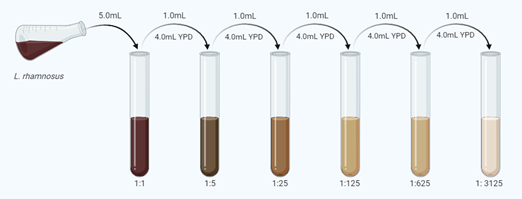
\includegraphics[width=0.75\linewidth]{Images/lram.png}
    \caption{Ratios used for serial dilutions}
    \label{fig:app_l_ram}
\end{figure}

\section{Glycerol Freezing}
The purpose of the glycerol freezing was to ensure the bacteria was preserved in a manner in which there would be limited growth and no death. This was done by letting the bacteria grow in the shaking incubator at $37^{\circ}C$ for 7 days. Afterwards, 32mL were extracted from the sample and centrifuged at 10,000g at $4^{\circ}C$ for 10 minutes in 2 50mL falcon tubes. 2 solutions of varying concentrations were created, with the first being a hyperconcentrated sample. This was done by extracting 17mL from the first tube resulting in a volume of 15mL + bacterial pellet. The pellet was resuspended in the 15mL by vortexing the sample. From this 3 solutions were created, 2 solutions of 5mL glycerol and 5mL sample, and 1 solution of 4mL glycerol and 4mL sample. For the second 32mL sample, none of the broth was removed to create a normal concentration. The pellet was resuspended in the 32mL by vortexing and 3 solutions of 5mL glycerol and 5mL sample. Afterwards, the tubes were all inverted and placed in a freezer at $-20^{\circ}C$. 


\section{Quartz Cuvette Spectral Interference}
The noise interference of the plastic cuvette was analyzed by comparing the spectra of ethanol and water when using a quartz cuvette. Figure 12 and Figure 13 show the spectra for ethanol and water in the different cuvettes. The spectra taken with the plastic cuvette showed a higher amount of noise than when taken with the quartz cuvette. The 1200 nm peak characteristic of ethanol has a flatter shape when the plastic cuvette is used. In contrast, the quartz cuvette shows a higher definition of this peak.

\begin{figure}[!h]
    \centering
    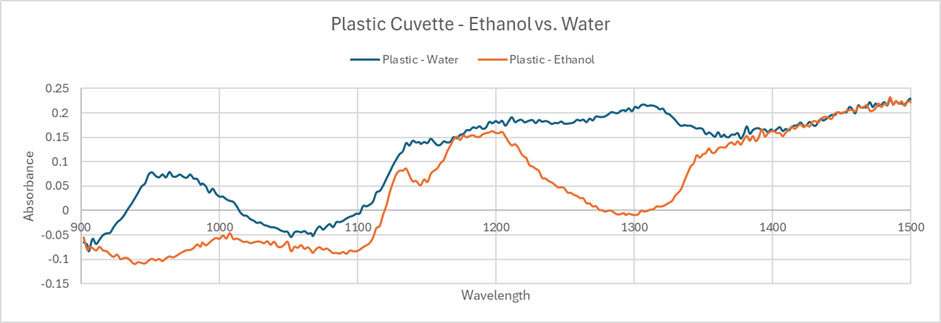
\includegraphics[width=0.75\linewidth]{Images/plastic_ew.png}
    \caption{Ethanol vs. Water Readings in a Quartz Cuvette}
    \label{fig:app_plastic}
\end{figure}

\begin{figure}[!h]
    \centering
    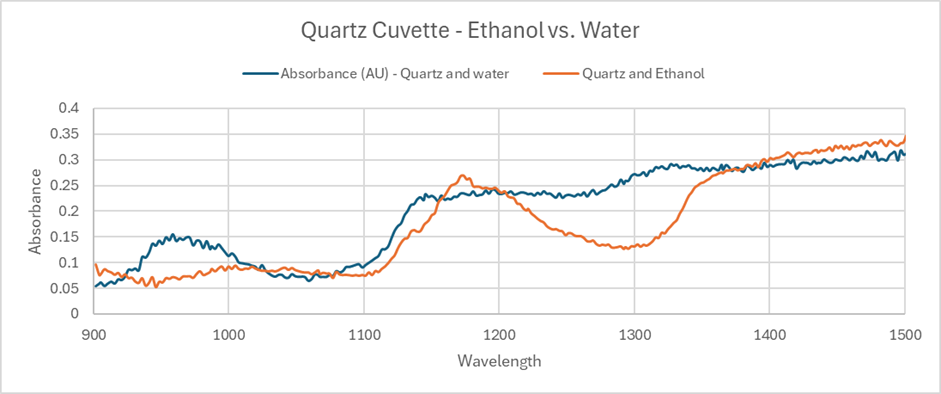
\includegraphics[width=0.75\linewidth]{Images/quartz_ew.png}
    \caption{Ethanol vs. Water Readings in a Quartz Cuvette}
    \label{fig:app_quartz}
\end{figure}

\section{Preliminary Training}
To allow for the construction of the model at the early stages of the project, the available data was used to train and validate the model’s performance. The small size of the training dataset represented a major problem for the accuracy of the model, the number of epochs, or cycles that the entire dataset passes through the algorithm during training, was adjusted to offset this limitation. The model was trained with 15 epochs to reduce the risk of overfitting, and an early stopping callback was included to stop the training process once the model showed no further improvement after each epoch. To ensure an efficient use of the limited dataset for both training and validation, cross-validation was implemented. This allowed for both the training and validation batch size to be 18, the total dataset size.

\subsection{One-Class Training}
The imbalanced data classes caused by the lack of data on contaminated samples resulted in the need to implement one-class training on the non-contaminated samples. This approach is commonly known as one-class classification or unary classification.\cite{brownlee_2020_oneclass} It enables the model to learn the characteristics of the “normal”, in this case, the non-contaminated samples, and subsequently classify between this data type and deviation from it, such as contaminated samples.

\subsection{K-Fold Cross-Validation}
To maximize the use of the limited data in both training and validation, as well as provide a more robust model evaluation, cross-validation was implemented with the K-fold method. This consists of splitting the dataset into k folds and using each fold once as a validation set while using the other folds for training. Due to the small dataset, the k was set to be 3 to maintain the same ratio of data per fold and maintain a balanced class distribution.

\addappendix{D}{Supplementary Results}

\begin{figure}[h]
    \centering
    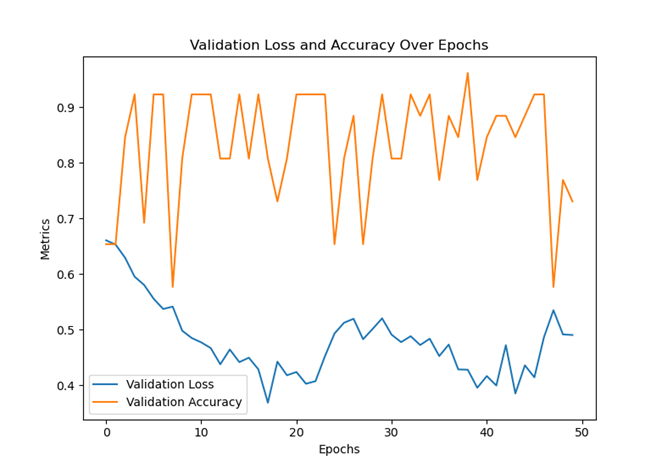
\includegraphics[width=0.75\linewidth]{Images/aa2.png}
    \caption{Validation loss and accuracy over 50 epochs. Model parameters remained the same throughout different training runs. Accuracy is unstable in a few training cases due to stratified sampling.}
    \label{fig:app_val_loss}
\end{figure}

\begin{figure}[h]
    \centering
    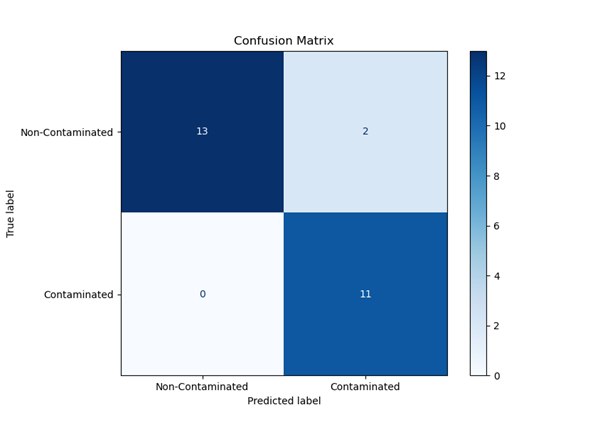
\includegraphics[width=0.75\linewidth]{Images/cm2.png}
    \caption{Confusion matrix of validation data. Poor discrimination accuracy observed in this run due to the randomly selected validation samples.}
    \label{fig:app_cm}
\end{figure}

\begin{figure}[h]
    \centering
    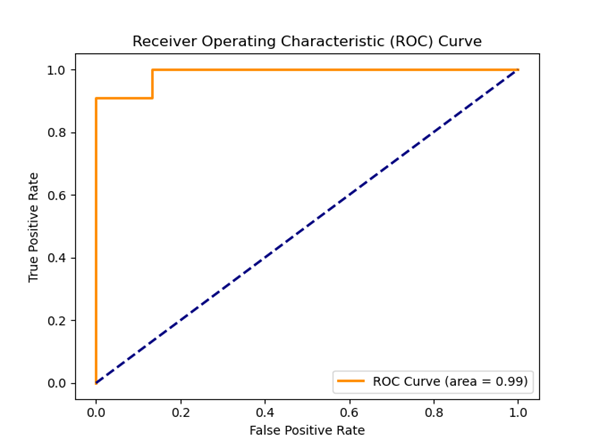
\includegraphics[width=0.75\linewidth]{Images/roc2.png}
    \caption{Receiver Operating Characteristic (ROC) curve for the model’s validation for a re-training run.}
    \label{fig:app_roc}
\end{figure}

\end{document}
